% Options for packages loaded elsewhere
\PassOptionsToPackage{unicode}{hyperref}
\PassOptionsToPackage{hyphens}{url}
\PassOptionsToPackage{dvipsnames,svgnames,x11names}{xcolor}
%
\documentclass[
]{article}

\usepackage{amsmath,amssymb}
\usepackage{iftex}
\ifPDFTeX
  \usepackage[T1]{fontenc}
  \usepackage[utf8]{inputenc}
  \usepackage{textcomp} % provide euro and other symbols
\else % if luatex or xetex
  \usepackage{unicode-math}
  \defaultfontfeatures{Scale=MatchLowercase}
  \defaultfontfeatures[\rmfamily]{Ligatures=TeX,Scale=1}
\fi
\usepackage{lmodern}
\ifPDFTeX\else  
    % xetex/luatex font selection
\fi
% Use upquote if available, for straight quotes in verbatim environments
\IfFileExists{upquote.sty}{\usepackage{upquote}}{}
\IfFileExists{microtype.sty}{% use microtype if available
  \usepackage[]{microtype}
  \UseMicrotypeSet[protrusion]{basicmath} % disable protrusion for tt fonts
}{}
\makeatletter
\@ifundefined{KOMAClassName}{% if non-KOMA class
  \IfFileExists{parskip.sty}{%
    \usepackage{parskip}
  }{% else
    \setlength{\parindent}{0pt}
    \setlength{\parskip}{6pt plus 2pt minus 1pt}}
}{% if KOMA class
  \KOMAoptions{parskip=half}}
\makeatother
\usepackage{xcolor}
\usepackage[margin=.75in]{geometry}
\setlength{\emergencystretch}{3em} % prevent overfull lines
\setcounter{secnumdepth}{-\maxdimen} % remove section numbering
% Make \paragraph and \subparagraph free-standing
\ifx\paragraph\undefined\else
  \let\oldparagraph\paragraph
  \renewcommand{\paragraph}[1]{\oldparagraph{#1}\mbox{}}
\fi
\ifx\subparagraph\undefined\else
  \let\oldsubparagraph\subparagraph
  \renewcommand{\subparagraph}[1]{\oldsubparagraph{#1}\mbox{}}
\fi


\providecommand{\tightlist}{%
  \setlength{\itemsep}{0pt}\setlength{\parskip}{0pt}}\usepackage{longtable,booktabs,array}
\usepackage{calc} % for calculating minipage widths
% Correct order of tables after \paragraph or \subparagraph
\usepackage{etoolbox}
\makeatletter
\patchcmd\longtable{\par}{\if@noskipsec\mbox{}\fi\par}{}{}
\makeatother
% Allow footnotes in longtable head/foot
\IfFileExists{footnotehyper.sty}{\usepackage{footnotehyper}}{\usepackage{footnote}}
\makesavenoteenv{longtable}
\usepackage{graphicx}
\makeatletter
\def\maxwidth{\ifdim\Gin@nat@width>\linewidth\linewidth\else\Gin@nat@width\fi}
\def\maxheight{\ifdim\Gin@nat@height>\textheight\textheight\else\Gin@nat@height\fi}
\makeatother
% Scale images if necessary, so that they will not overflow the page
% margins by default, and it is still possible to overwrite the defaults
% using explicit options in \includegraphics[width, height, ...]{}
\setkeys{Gin}{width=\maxwidth,height=\maxheight,keepaspectratio}
% Set default figure placement to htbp
\makeatletter
\def\fps@figure{htbp}
\makeatother

\usepackage{booktabs}
\usepackage{caption}
\usepackage{longtable}
\usepackage{colortbl}
\usepackage{array}
\usepackage{geometry}
\usepackage{pdflscape}
\usepackage{caption}
\captionsetup{labelfont=bf, textfont=normalfont, justification=raggedright, singlelinecheck=false}
\makeatletter
\renewcommand{\fnum@figure}{\figurename\thefigure}
\renewcommand{\fnum@table}{\tablename\thetable}
\makeatother
\pagenumbering{gobble}
\makeatletter
\makeatother
\makeatletter
\makeatother
\makeatletter
\@ifpackageloaded{caption}{}{\usepackage{caption}}
\AtBeginDocument{%
\ifdefined\contentsname
  \renewcommand*\contentsname{Table of contents}
\else
  \newcommand\contentsname{Table of contents}
\fi
\ifdefined\listfigurename
  \renewcommand*\listfigurename{List of Figures}
\else
  \newcommand\listfigurename{List of Figures}
\fi
\ifdefined\listtablename
  \renewcommand*\listtablename{List of Tables}
\else
  \newcommand\listtablename{List of Tables}
\fi
\ifdefined\figurename
  \renewcommand*\figurename{Supplementary Figure S}
\else
  \newcommand\figurename{Supplementary Figure S}
\fi
\ifdefined\tablename
  \renewcommand*\tablename{Supplementary Table S}
\else
  \newcommand\tablename{Supplementary Table S}
\fi
}
\@ifpackageloaded{float}{}{\usepackage{float}}
\floatstyle{ruled}
\@ifundefined{c@chapter}{\newfloat{codelisting}{h}{lop}}{\newfloat{codelisting}{h}{lop}[chapter]}
\floatname{codelisting}{Listing}
\newcommand*\listoflistings{\listof{codelisting}{List of Listings}}
\makeatother
\makeatletter
\@ifpackageloaded{caption}{}{\usepackage{caption}}
\@ifpackageloaded{subcaption}{}{\usepackage{subcaption}}
\makeatother
\makeatletter
\@ifpackageloaded{tcolorbox}{}{\usepackage[skins,breakable]{tcolorbox}}
\makeatother
\makeatletter
\@ifundefined{shadecolor}{\definecolor{shadecolor}{rgb}{.97, .97, .97}}
\makeatother
\makeatletter
\makeatother
\makeatletter
\makeatother
\ifLuaTeX
  \usepackage{selnolig}  % disable illegal ligatures
\fi
\IfFileExists{bookmark.sty}{\usepackage{bookmark}}{\usepackage{hyperref}}
\IfFileExists{xurl.sty}{\usepackage{xurl}}{} % add URL line breaks if available
\urlstyle{same} % disable monospaced font for URLs
\hypersetup{
  pdftitle={Supplementary Materials},
  colorlinks=true,
  linkcolor={blue},
  filecolor={Maroon},
  citecolor={Blue},
  urlcolor={Blue},
  pdfcreator={LaTeX via pandoc}}

\title{Supplementary Materials}
\author{}
\date{}

\begin{document}
\maketitle
\ifdefined\Shaded\renewenvironment{Shaded}{\begin{tcolorbox}[sharp corners, borderline west={3pt}{0pt}{shadecolor}, interior hidden, breakable, boxrule=0pt, frame hidden, enhanced]}{\end{tcolorbox}}\fi

\begin{figure}[H]

{\centering 
\includegraphics[width=0.9\textwidth,height=\textheight]{fig S1 - exp1 invsimpson.pdf}

}

\caption{\label{fig-s1}Alpha diversity across storage conditions in the
first experiment. Bar plots showing sample-level alpha diversity for the
first experiment, as measured by the Inverse Simpson index. Samples are
organized by storage temperature and storage duration, as indicated by
the facet labels above each panel. ANOVA results for storage
temperature, storage duration, and their interaction are shown below the
plot.}

\end{figure}

\newpage

\begin{figure}[H]

{\centering 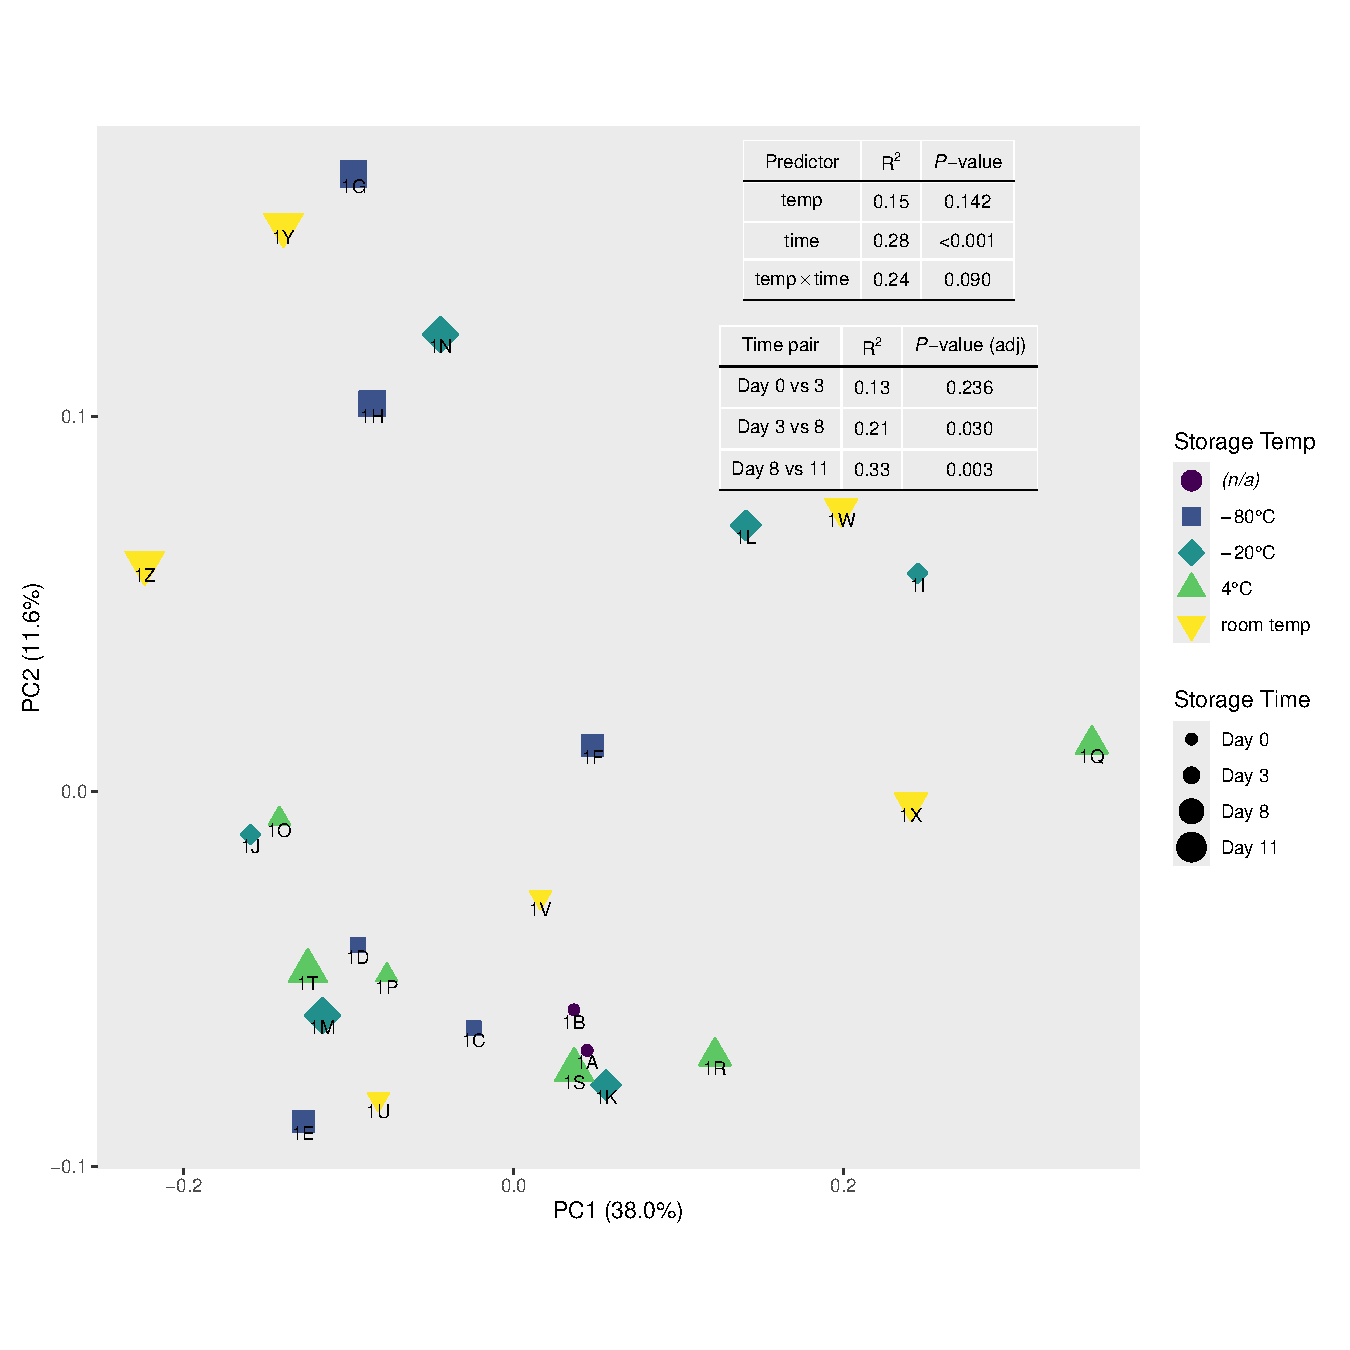
\includegraphics[width=0.7\textwidth,height=\textheight]{fig S2 - exp1 pcoa permanova bray.pdf}

}

\caption{\label{fig-s2}Principal coordinate analysis of Bray--Curtis
distances across storage conditions in the first experiment. Principal
coordinate analysis (PCoA) plot based on Bray--Curtis distances between
samples in the first experiment. Colors indicate storage duration, and
shapes indicate storage temperature. Inset tables summarize PERMANOVA
results for storage temperature, storage duration, and their
interaction, along with pairwise comparisons between storage durations.
Percent variation explained for each axis is indicated in parentheses.}

\end{figure}

\newpage

\begin{figure}[H]

{\centering 
\includegraphics[width=0.9\textwidth,height=\textheight]{fig S3 - exp1 qPCR.pdf}

}

\caption{\label{fig-s3}Absolute bacterial abundance measured by 16S qPCR
across storage conditions in the first experiment. Bar plot showing
absolute bacterial abundance measured by 16S qPCR across all
first-experiment samples. Samples are grouped by storage temperature and
duration, as indicated by the facet labels above each panel. The y-axis
is displayed on a logarithmic scale. Inset text summarizes ANOVA results
for storage temperature, storage duration, and their interaction, along
with pairwise comparisons between storage durations.}

\end{figure}

\newpage
\pdfpagewidth=16in
\pdfpageheight=12in
\newgeometry{margin=0.75in}

\begin{figure}[H]

{\centering 
\includegraphics[width=16in,height=\textheight]{fig S4 - exp1 step all.pdf}

}

\caption{\label{fig-s4}Taxon-level relative abundance shifts relative to
the baseline sample in the first experiment. Rank relative abundance
plots showing taxon-level composition of all first experiment samples
compared with the baseline sample, 1A (blue dashed box). Taxa are
ordered by relative abundance in the baseline sample. Colored bars
represent taxon abundances in each comparison sample, with colors
indicating taxonomic classification. The black overlay line shows the
baseline abundance profile for the same ordered taxa. Blue labels
indicate the Morisita--Horn distance between each comparison sample and
baseline.}

\end{figure}

\newpage
\pdfpagewidth=8.5in
\pdfpageheight=11in
\restoregeometry

\begin{figure}[H]

{\centering 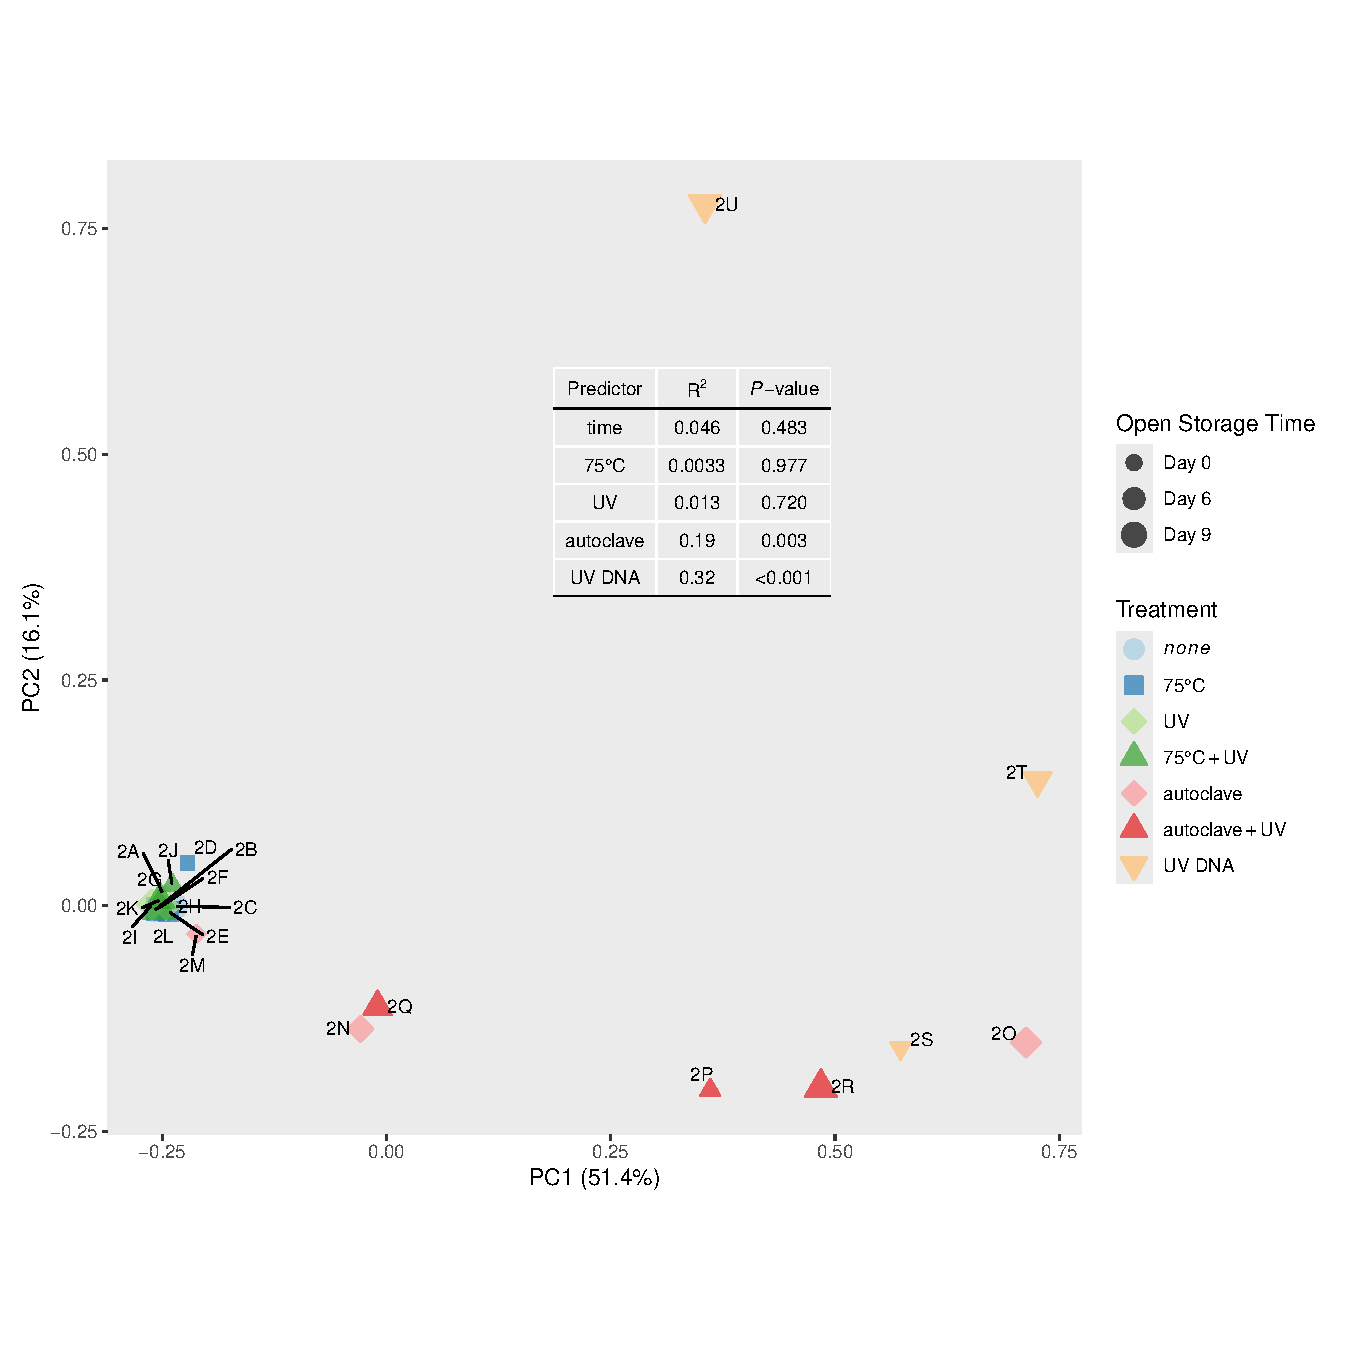
\includegraphics[width=0.7\textwidth,height=\textheight]{fig S5 - exp2 pcoa permanova bray.pdf}

}

\caption{\label{fig-s5}Principal coordinate analysis of Bray--Curtis
distances across storage durations and treatments in the second
experiment. Principal coordinate analysis (PCoA) plot based on
Bray--Curtis distances between samples in the second experiment. Colors
indicate storage duration, and shapes indicate storage temperature.
Inset tables summarize PERMANOVA results for 75 °C heat treatment, UV
exposure before DNA extraction, UV exposure after DNA extraction, and
pre-extraction autoclaving. Percent variation explained for each axis is
indicated in parentheses.}

\end{figure}

\newpage

\begin{figure}[H]

{\centering 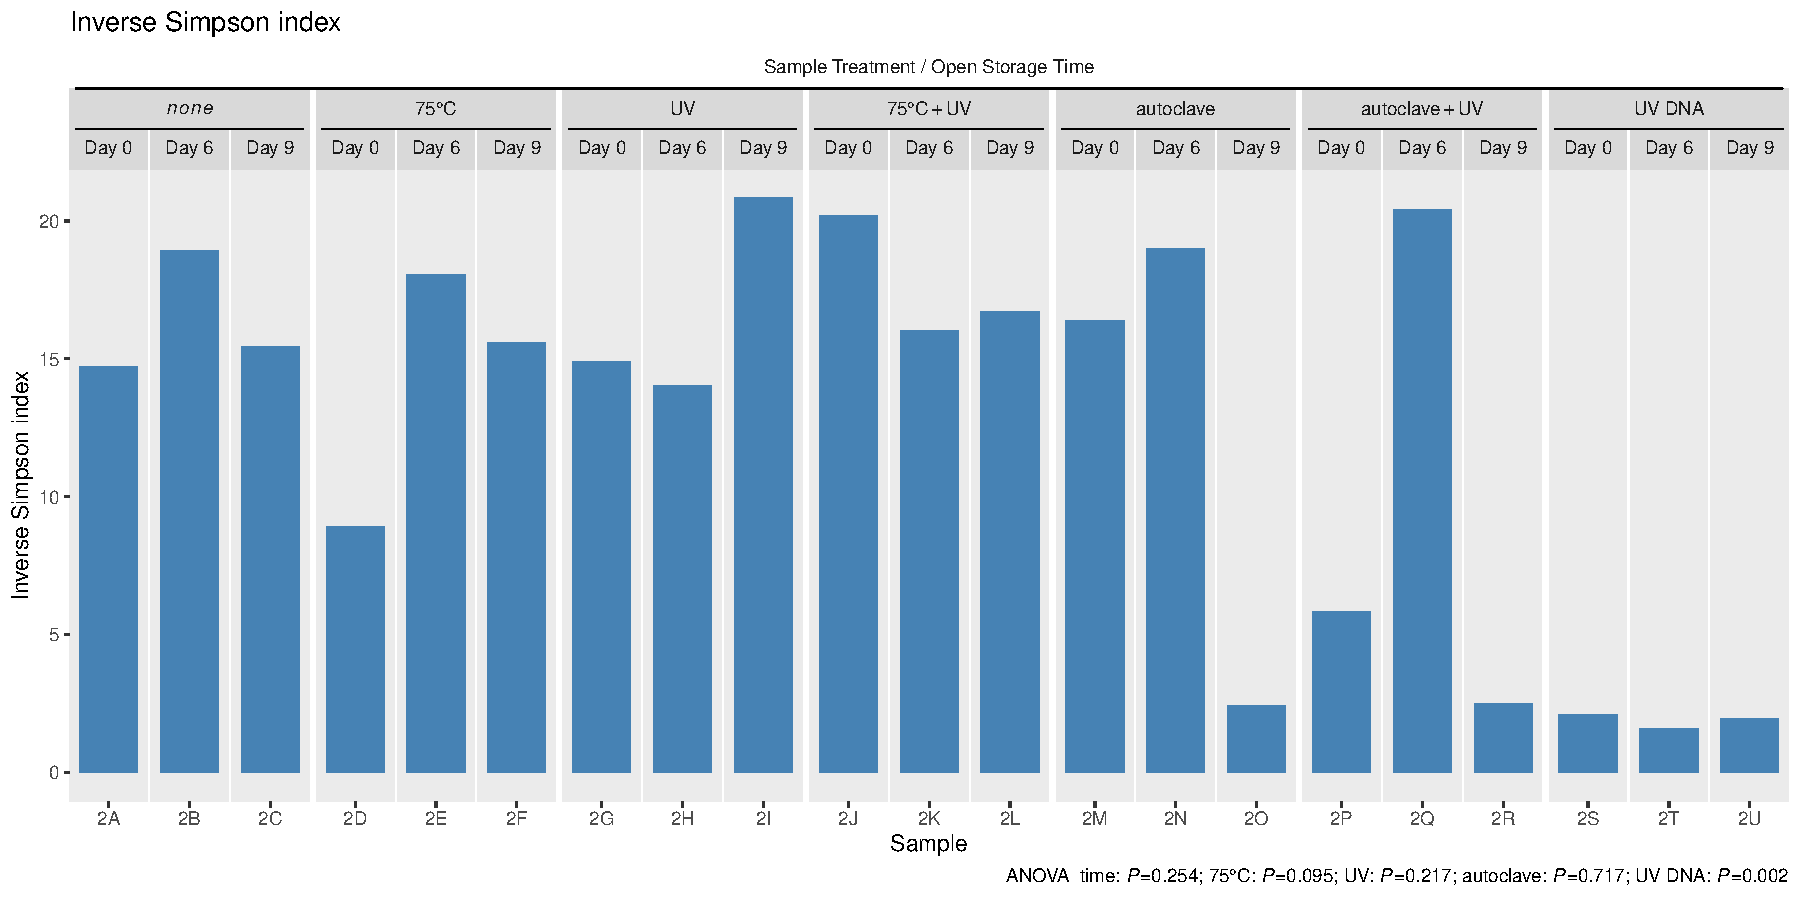
\includegraphics[width=0.9\textwidth,height=\textheight]{fig S6 - exp2 invsimpson.pdf}

}

\caption{\label{fig-s6}Alpha diversity across storage durations and
treatments in the second experiment. Bar plots showing sample-level
alpha diversity for the second experiment, as measured by the Inverse
Simpson index. Samples are organized by treatment and storage duration,
as indicated by the facet labels above each panel. ANOVA results
evaluating the effects of storage duration, 75 °C heat treatment, UV
exposure before DNA extraction, UV exposure after DNA extraction, and
pre-extraction autoclaving are shown below the plot.}

\end{figure}

\newpage

\begin{figure}[H]

{\centering 
\includegraphics[width=0.9\textwidth,height=\textheight]{fig S7 - exp2 qpcr.pdf}

}

\caption{\label{fig-s7}Absolute bacterial abundance measured by 16S qPCR
across storage durations and treatments in the second experiment. Bar
plot showing absolute bacterial abundance measured by 16S qPCR across
all second-experiment samples. Samples are grouped by treatment and
storage duration, as indicated by the facet labels above each panel.
ANOVA results evaluating the effects of storage duration, 75 °C heat
treatment, UV exposure before DNA extraction, UV exposure after DNA
extraction, and pre-extraction autoclaving are shown below the plot.}

\end{figure}

\newpage

\begin{figure}[H]

{\centering 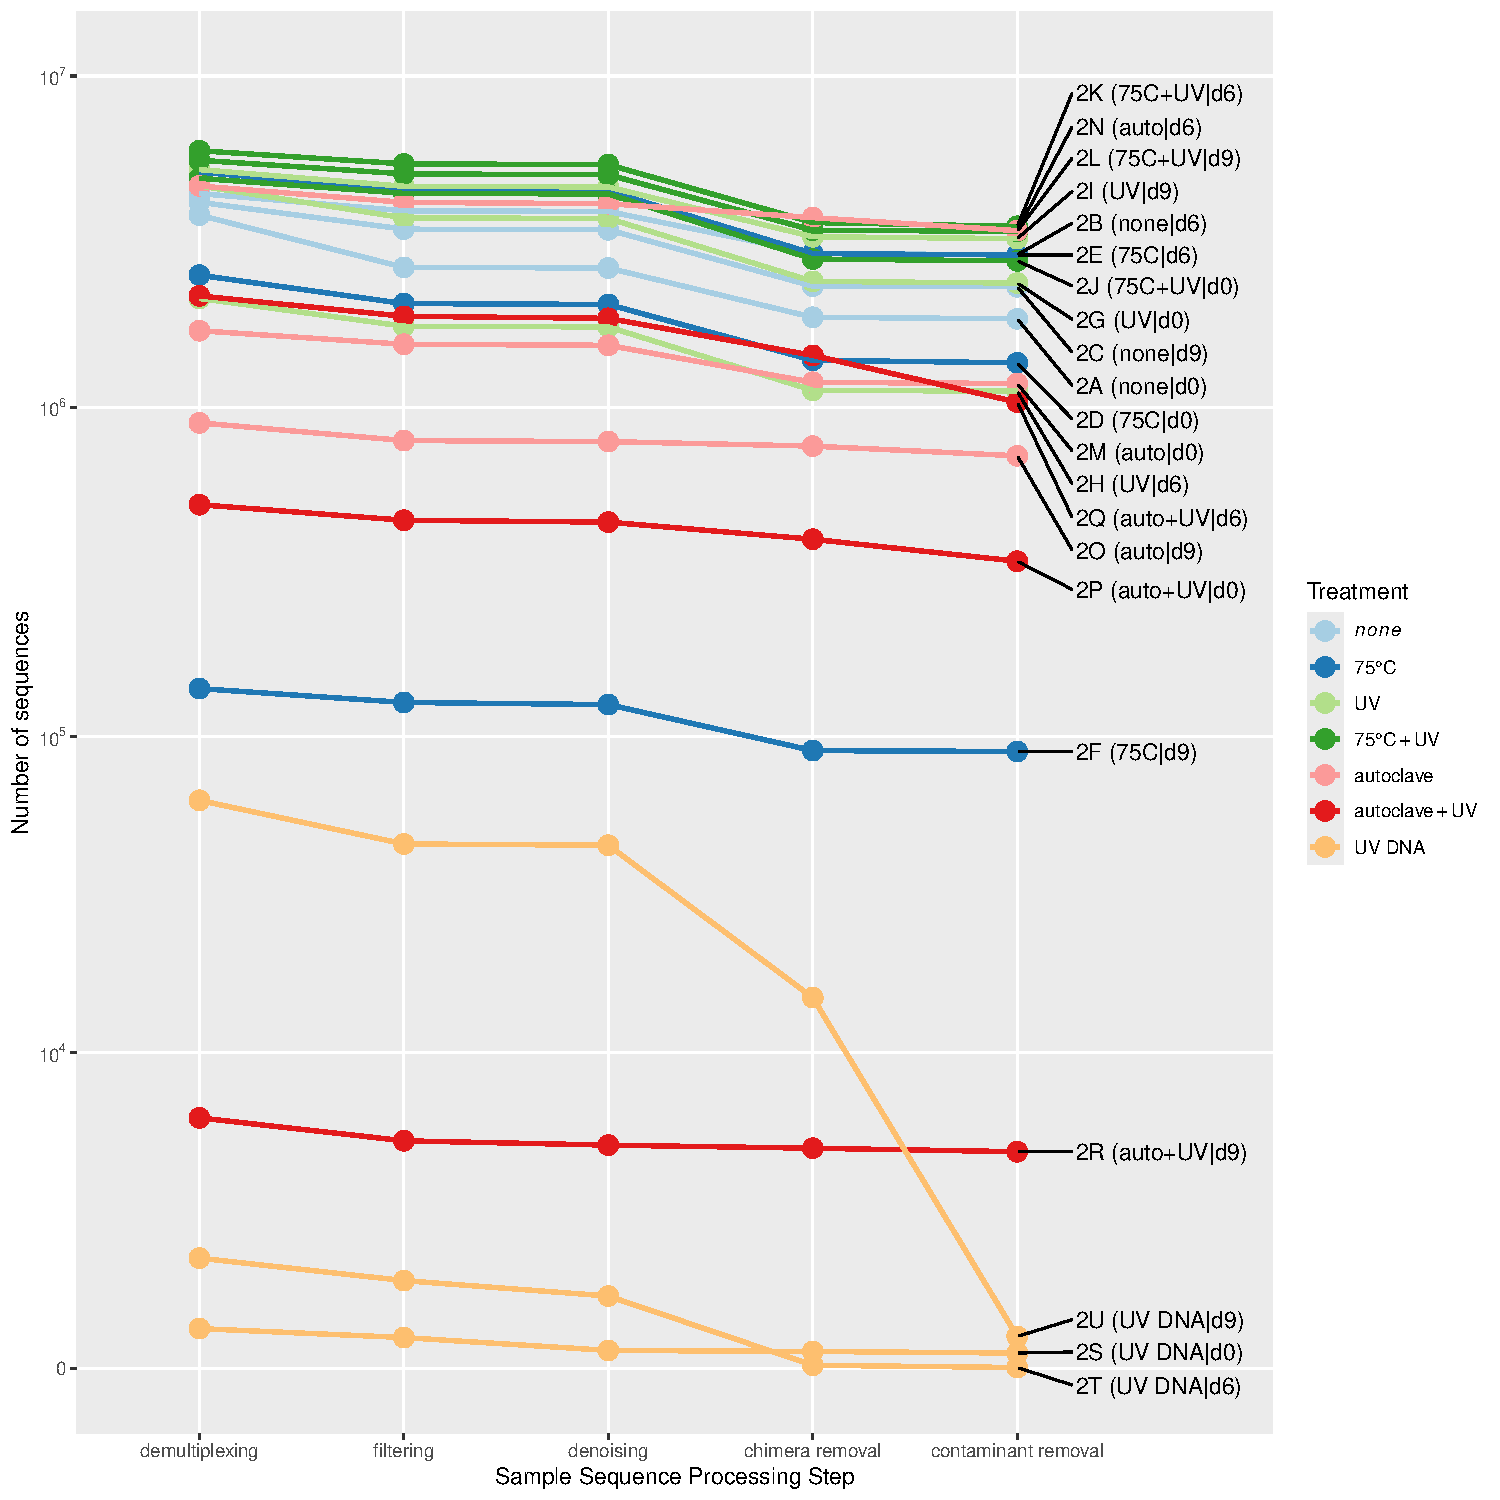
\includegraphics[width=1\textwidth,height=\textheight]{fig S8 - exp2 seqloss.pdf}

}

\caption{\label{fig-s8}Read retention across sequence-processing steps
in the second experiment. Line plot showing the number of sequences
retained for each second-experiment sample across sequential DADA2
processing steps, including demultiplexing, filtering, denoising,
chimera removal, and contaminant removal. Lines represent individual
samples and are colored by treatment condition. Sample labels are shown
at the final processing step.}

\end{figure}

\newpage
\pdfpagewidth=19in
\pdfpageheight=11in
\newgeometry{margin=0.5in}

\begin{figure}[H]

{\centering 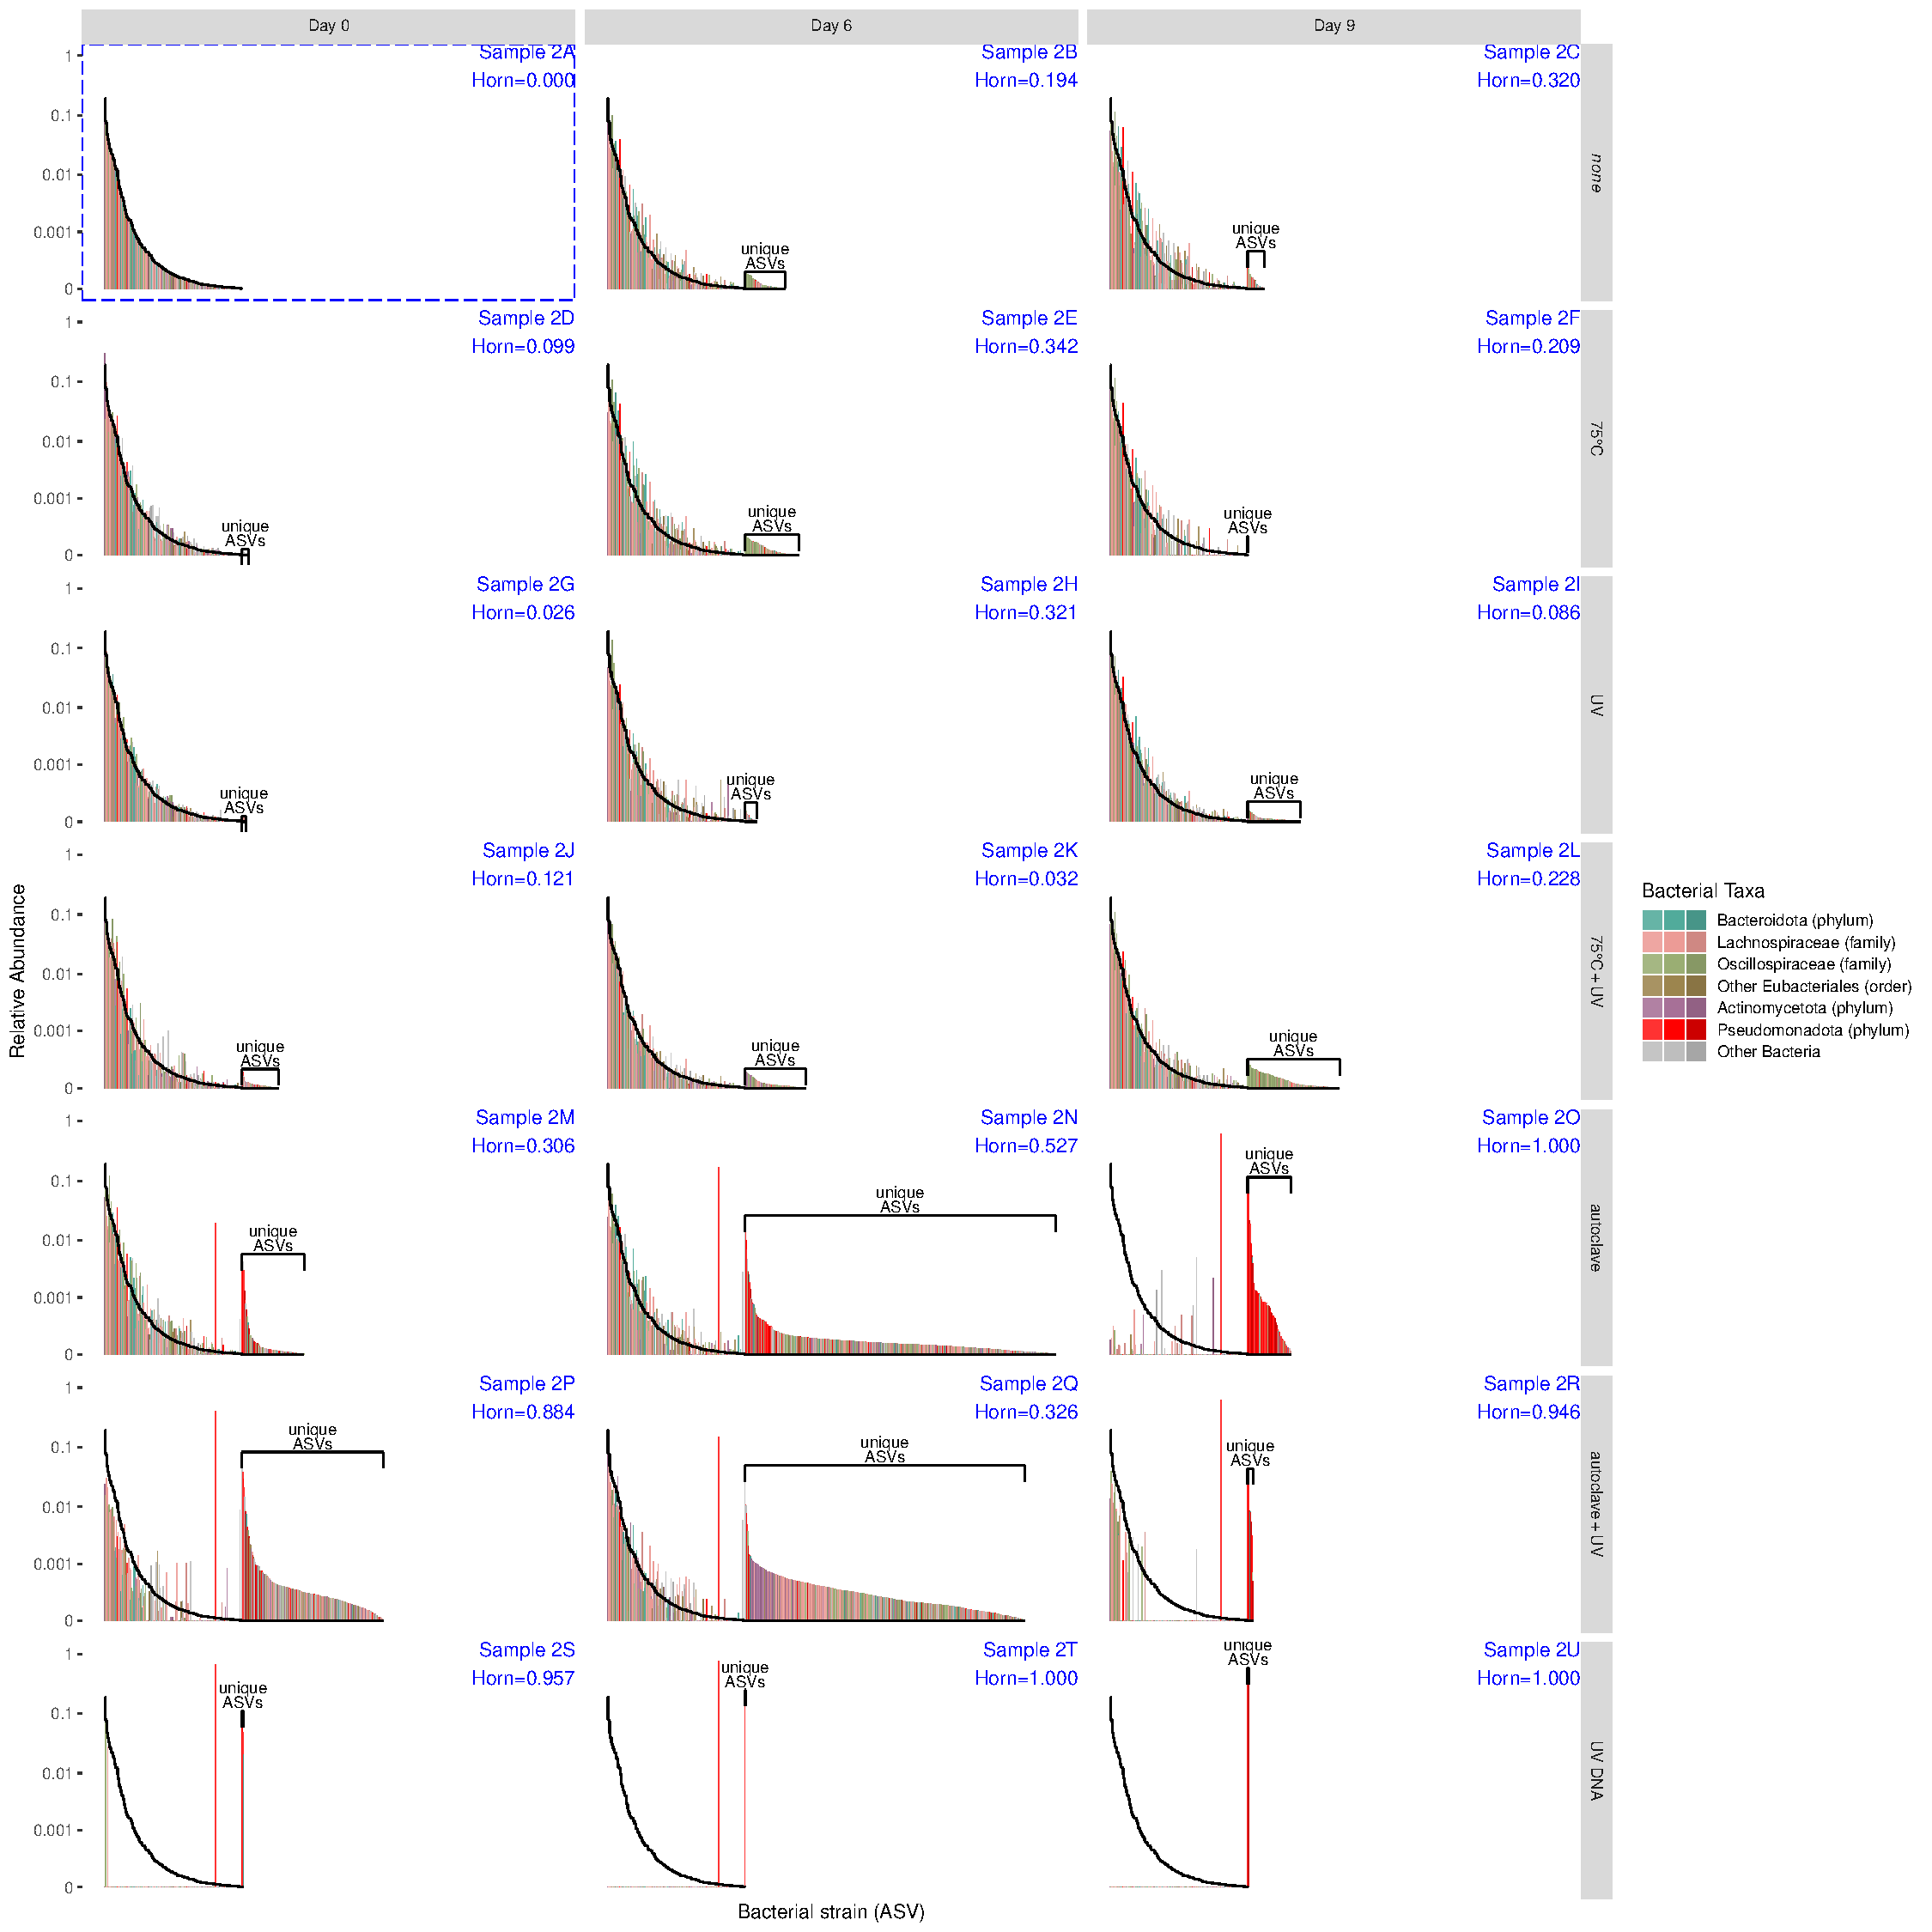
\includegraphics[width=18in,height=\textheight]{fig S9 - exp2 step all.pdf}

}

\caption{\label{fig-s9}Taxon-level relative abundance shifts relative to
the baseline sample in the second experiment. Rank relative abundance
plots showing taxon-level composition of all second experiment samples
compared with the baseline sample, 2A (blue dashed box). Taxa are
ordered by relative abundance in the baseline sample. Colored bars
represent taxon abundances in each comparison sample, with colors
indicating taxonomic classification. The black overlay line shows the
baseline abundance profile for the same ordered taxa. Blue labels
indicate the Morisita--Horn distance between each comparison sample and
baseline.}

\end{figure}

\newpage
\pdfpagewidth=14in
\pdfpageheight=8.5in
\newgeometry{margin=0.5in}

\hypertarget{tbl-s1}{}
\begin{longtable}{l|clrrr}
\caption{\label{tbl-s1}Linear discriminant analysis effect size (LEfSe) results comparing
samples stored for 0--8 days with samples stored for 11 days. The
Direction column indicates the group in which each taxon was enriched.
Taxonomic assignments are shown with the corresponding rank, LDA score,
and Kruskal--Wallis p-value. LDA, linear discriminant analysis; KW,
Kruskal--Wallis }\tabularnewline

\caption*{
{\large Predictors of Storage Time}
} \\ 
\toprule
\multicolumn{1}{l}{Direction} & Rank & Taxonomy & LDA & KW \emph{P}-value & Log-Max \\ 
\midrule\addlinespace[2.5pt]
\cellcolor[HTML]{D9F1FF}{Day 0-8} & \cellcolor[HTML]{D9F1FF}{(4) Order} & \cellcolor[HTML]{D9F1FF}{Bacteria|Bacillota|Clostridia|Eubacteriales} & \cellcolor[HTML]{D9F1FF}{$4.53$} & \cellcolor[HTML]{D9F1FF}{0.020} & \cellcolor[HTML]{D9F1FF}{$5.45$} \\ 
 & \cellcolor[HTML]{D9F1FF}{(5) Family} & \cellcolor[HTML]{D9F1FF}{Bacteria|Bacillota|Clostridia|Eubacteriales|Oscillospiraceae} & \cellcolor[HTML]{D9F1FF}{$4.63$} & \cellcolor[HTML]{D9F1FF}{0.006} & \cellcolor[HTML]{D9F1FF}{$5.37$} \\ 
 & \cellcolor[HTML]{D9F1FF}{(6) Genus} & \cellcolor[HTML]{D9F1FF}{Bacteria|Bacillota|Clostridia|Eubacteriales|Oscillospiraceae|Faecalibacterium} & \cellcolor[HTML]{D9F1FF}{$4.58$} & \cellcolor[HTML]{D9F1FF}{0.009} & \cellcolor[HTML]{D9F1FF}{$5.29$} \\ 
 & \cellcolor[HTML]{D9F1FF}{(7) Species} & \cellcolor[HTML]{D9F1FF}{Bacteria|Bacillota|Clostridia|Eubacteriales|Oscillospiraceae|Faecalibacterium|Faecalibacterium prausnitzii} & \cellcolor[HTML]{D9F1FF}{$4.58$} & \cellcolor[HTML]{D9F1FF}{0.009} & \cellcolor[HTML]{D9F1FF}{$5.29$} \\ 
 & \cellcolor[HTML]{D9F1FF}{(6) Genus} & \cellcolor[HTML]{D9F1FF}{Bacteria|Bacillota|Clostridia|Eubacteriales|Oscillospiraceae|Ruminococcus} & \cellcolor[HTML]{D9F1FF}{$3.45$} & \cellcolor[HTML]{D9F1FF}{<0.001} & \cellcolor[HTML]{D9F1FF}{$4.06$} \\ 
 & \cellcolor[HTML]{D9F1FF}{(7) Species} & \cellcolor[HTML]{D9F1FF}{Bacteria|Bacillota|Clostridia|Eubacteriales|Oscillospiraceae|Ruminococcus|Ruminococcus champanellensis} & \cellcolor[HTML]{D9F1FF}{$3.45$} & \cellcolor[HTML]{D9F1FF}{<0.001} & \cellcolor[HTML]{D9F1FF}{$4.06$} \\ 
 & \cellcolor[HTML]{D9F1FF}{(7) Species} & \cellcolor[HTML]{D9F1FF}{Bacteria|Bacillota|Clostridia|Eubacteriales|Oscillospiraceae|—|Clostridium leptum} & \cellcolor[HTML]{D9F1FF}{$3.06$} & \cellcolor[HTML]{D9F1FF}{0.030} & \cellcolor[HTML]{D9F1FF}{$3.81$} \\ 
 & \cellcolor[HTML]{D9F1FF}{(6) Genus} & \cellcolor[HTML]{D9F1FF}{Bacteria|Bacillota|Clostridia|Eubacteriales|—|Gemmiger} & \cellcolor[HTML]{D9F1FF}{$3.71$} & \cellcolor[HTML]{D9F1FF}{<0.001} & \cellcolor[HTML]{D9F1FF}{$4.42$} \\ 
 & \cellcolor[HTML]{D9F1FF}{(7) Species} & \cellcolor[HTML]{D9F1FF}{Bacteria|Bacillota|Clostridia|Eubacteriales|—|Gemmiger|Gemmiger formicilis} & \cellcolor[HTML]{D9F1FF}{$3.71$} & \cellcolor[HTML]{D9F1FF}{<0.001} & \cellcolor[HTML]{D9F1FF}{$4.42$} \\ 
 & \cellcolor[HTML]{D9F1FF}{(6) Genus} & \cellcolor[HTML]{D9F1FF}{Bacteria|Bacillota|Clostridia|Lachnospirales|Lachnospiraceae|Agathobacter} & \cellcolor[HTML]{D9F1FF}{$3.79$} & \cellcolor[HTML]{D9F1FF}{0.009} & \cellcolor[HTML]{D9F1FF}{$4.47$} \\ 
 & \cellcolor[HTML]{D9F1FF}{(7) Species} & \cellcolor[HTML]{D9F1FF}{Bacteria|Bacillota|Clostridia|Lachnospirales|Lachnospiraceae|Agathobacter|Agathobacter rectalis} & \cellcolor[HTML]{D9F1FF}{$3.79$} & \cellcolor[HTML]{D9F1FF}{0.009} & \cellcolor[HTML]{D9F1FF}{$4.47$} \\ 
 & \cellcolor[HTML]{D9F1FF}{(2) Phylum} & \cellcolor[HTML]{D9F1FF}{Bacteria|Pseudomonadota} & \cellcolor[HTML]{D9F1FF}{$4.04$} & \cellcolor[HTML]{D9F1FF}{0.035} & \cellcolor[HTML]{D9F1FF}{$4.63$} \\ 
 & \cellcolor[HTML]{D9F1FF}{(3) Class} & \cellcolor[HTML]{D9F1FF}{Bacteria|Pseudomonadota|Betaproteobacteria} & \cellcolor[HTML]{D9F1FF}{$4.07$} & \cellcolor[HTML]{D9F1FF}{0.011} & \cellcolor[HTML]{D9F1FF}{$4.61$} \\ 
 & \cellcolor[HTML]{D9F1FF}{(4) Order} & \cellcolor[HTML]{D9F1FF}{Bacteria|Pseudomonadota|Betaproteobacteria|Burkholderiales} & \cellcolor[HTML]{D9F1FF}{$4.07$} & \cellcolor[HTML]{D9F1FF}{0.011} & \cellcolor[HTML]{D9F1FF}{$4.61$} \\ 
 & \cellcolor[HTML]{D9F1FF}{(5) Family} & \cellcolor[HTML]{D9F1FF}{Bacteria|Pseudomonadota|Betaproteobacteria|Burkholderiales|Sutterellaceae} & \cellcolor[HTML]{D9F1FF}{$4.07$} & \cellcolor[HTML]{D9F1FF}{0.011} & \cellcolor[HTML]{D9F1FF}{$4.61$} \\ 
 & \cellcolor[HTML]{D9F1FF}{(6) Genus} & \cellcolor[HTML]{D9F1FF}{Bacteria|Pseudomonadota|Betaproteobacteria|Burkholderiales|Sutterellaceae|Parasutterella} & \cellcolor[HTML]{D9F1FF}{$4.07$} & \cellcolor[HTML]{D9F1FF}{0.011} & \cellcolor[HTML]{D9F1FF}{$4.61$} \\ 
 & \cellcolor[HTML]{D9F1FF}{(7) Species} & \cellcolor[HTML]{D9F1FF}{Bacteria|Pseudomonadota|Betaproteobacteria|Burkholderiales|Sutterellaceae|Parasutterella|Parasutterella excrementihominis} & \cellcolor[HTML]{D9F1FF}{$4.07$} & \cellcolor[HTML]{D9F1FF}{0.011} & \cellcolor[HTML]{D9F1FF}{$4.61$} \\ 
\midrule\addlinespace[2.5pt]
\cellcolor[HTML]{FFE0DB}{Day 11} & \cellcolor[HTML]{FFE0DB}{(7) Species} & \cellcolor[HTML]{FFE0DB}{Bacteria|Actinomycetota|Actinomycetes|Bifidobacteriales|Bifidobacteriaceae|Bifidobacterium|Bifidobacterium longum} & \cellcolor[HTML]{FFE0DB}{$4.12$} & \cellcolor[HTML]{FFE0DB}{0.023} & \cellcolor[HTML]{FFE0DB}{$4.96$} \\ 
 & \cellcolor[HTML]{FFE0DB}{(5) Family} & \cellcolor[HTML]{FFE0DB}{Bacteria|Bacillota|Clostridia|Eubacteriales|Clostridiaceae} & \cellcolor[HTML]{FFE0DB}{$4.15$} & \cellcolor[HTML]{FFE0DB}{0.005} & \cellcolor[HTML]{FFE0DB}{$4.60$} \\ 
 & \cellcolor[HTML]{FFE0DB}{(6) Genus} & \cellcolor[HTML]{FFE0DB}{Bacteria|Bacillota|Clostridia|Eubacteriales|Clostridiaceae|Clostridium} & \cellcolor[HTML]{FFE0DB}{$4.15$} & \cellcolor[HTML]{FFE0DB}{0.006} & \cellcolor[HTML]{FFE0DB}{$4.60$} \\ 
 & \cellcolor[HTML]{FFE0DB}{(7) Species} & \cellcolor[HTML]{FFE0DB}{Bacteria|Bacillota|Clostridia|Eubacteriales|Clostridiaceae|Clostridium|Clostridium innocuum} & \cellcolor[HTML]{FFE0DB}{$4.15$} & \cellcolor[HTML]{FFE0DB}{0.005} & \cellcolor[HTML]{FFE0DB}{$4.59$} \\ 
 & \cellcolor[HTML]{FFE0DB}{(6) Genus} & \cellcolor[HTML]{FFE0DB}{Bacteria|Bacillota|Clostridia|Lachnospirales|Lachnospiraceae|Tyzzerella} & \cellcolor[HTML]{FFE0DB}{$4.17$} & \cellcolor[HTML]{FFE0DB}{0.035} & \cellcolor[HTML]{FFE0DB}{$4.73$} \\ 
 & \cellcolor[HTML]{FFE0DB}{(7) Species} & \cellcolor[HTML]{FFE0DB}{Bacteria|Bacillota|Clostridia|Lachnospirales|Lachnospiraceae|Tyzzerella|Clostridium nexile} & \cellcolor[HTML]{FFE0DB}{$4.17$} & \cellcolor[HTML]{FFE0DB}{0.035} & \cellcolor[HTML]{FFE0DB}{$4.73$} \\ 
 & \cellcolor[HTML]{FFE0DB}{(3) Class} & \cellcolor[HTML]{FFE0DB}{Bacteria|Bacillota|Erysipelotrichia} & \cellcolor[HTML]{FFE0DB}{$3.90$} & \cellcolor[HTML]{FFE0DB}{0.046} & \cellcolor[HTML]{FFE0DB}{$4.64$} \\ 
 & \cellcolor[HTML]{FFE0DB}{(4) Order} & \cellcolor[HTML]{FFE0DB}{Bacteria|Bacillota|Erysipelotrichia|Erysipelotrichales} & \cellcolor[HTML]{FFE0DB}{$3.90$} & \cellcolor[HTML]{FFE0DB}{0.046} & \cellcolor[HTML]{FFE0DB}{$4.64$} \\ 
 & \cellcolor[HTML]{FFE0DB}{(5) Family} & \cellcolor[HTML]{FFE0DB}{Bacteria|Bacillota|Erysipelotrichia|Erysipelotrichales|Coprobacillaceae} & \cellcolor[HTML]{FFE0DB}{$3.89$} & \cellcolor[HTML]{FFE0DB}{0.035} & \cellcolor[HTML]{FFE0DB}{$4.58$} \\ 
 & \cellcolor[HTML]{FFE0DB}{(6) Genus} & \cellcolor[HTML]{FFE0DB}{Bacteria|Bacillota|Erysipelotrichia|Erysipelotrichales|Coprobacillaceae|Coprobacillus} & \cellcolor[HTML]{FFE0DB}{$3.33$} & \cellcolor[HTML]{FFE0DB}{0.023} & \cellcolor[HTML]{FFE0DB}{$3.85$} \\ 
 & \cellcolor[HTML]{FFE0DB}{(7) Species} & \cellcolor[HTML]{FFE0DB}{Bacteria|Bacillota|Erysipelotrichia|Erysipelotrichales|Coprobacillaceae|Coprobacillus|Coprobacillus cateniformis} & \cellcolor[HTML]{FFE0DB}{$3.33$} & \cellcolor[HTML]{FFE0DB}{0.023} & \cellcolor[HTML]{FFE0DB}{$3.85$} \\ 
 & \cellcolor[HTML]{FFE0DB}{(3) Class} & \cellcolor[HTML]{FFE0DB}{Bacteria|Bacillota|Tissierellia} & \cellcolor[HTML]{FFE0DB}{$3.32$} & \cellcolor[HTML]{FFE0DB}{0.035} & \cellcolor[HTML]{FFE0DB}{$3.73$} \\ 
 & \cellcolor[HTML]{FFE0DB}{(4) Order} & \cellcolor[HTML]{FFE0DB}{Bacteria|Bacillota|Tissierellia|Tissierellales} & \cellcolor[HTML]{FFE0DB}{$3.32$} & \cellcolor[HTML]{FFE0DB}{0.035} & \cellcolor[HTML]{FFE0DB}{$3.73$} \\ 
 & \cellcolor[HTML]{FFE0DB}{(5) Family} & \cellcolor[HTML]{FFE0DB}{Bacteria|Bacillota|Tissierellia|Tissierellales|Peptoniphilaceae} & \cellcolor[HTML]{FFE0DB}{$3.32$} & \cellcolor[HTML]{FFE0DB}{0.035} & \cellcolor[HTML]{FFE0DB}{$3.73$} \\ 
\bottomrule
\end{longtable}

\newpage
\pdfpagewidth=14in
\pdfpageheight=25in
\newgeometry{margin=0.5in}

\begin{table}

\caption{\label{tbl-s2a}Linear discriminant analysis effect size (LEfSe)
results are shown for two comparisons: autoclaved samples versus
untreated samples, and UV-DNA irradiated samples versus untreated
samples. The Direction column indicates the group in which each taxon
was enriched. Taxonomic assignments are shown with the corresponding
rank, LDA score, and Kruskal--Wallis p-value. LDA, linear discriminant
analysis; KW, Kruskal--Wallis.}\begin{minipage}[t]{\linewidth}
\subcaption{\label{tbl-s2a-1}}

{\centering 

\begin{longtable*}{l|clrrr}
\caption*{
{\large Predictors of autoclave vs. no treatment}
} \\ 
\toprule
\multicolumn{1}{l}{Direction} & Rank & Taxonomy & LDA & KW \emph{P}-value & Log-Max \\ 
\midrule\addlinespace[2.5pt]
\cellcolor[HTML]{D9F1FF}{autoclave} & \cellcolor[HTML]{D9F1FF}{(3) Class} & \cellcolor[HTML]{D9F1FF}{Bacteria|Bacteroidota|Flavobacteriia} & \cellcolor[HTML]{D9F1FF}{$3.22$} & \cellcolor[HTML]{D9F1FF}{0.037} & \cellcolor[HTML]{D9F1FF}{$3.52$} \\ 
 & \cellcolor[HTML]{D9F1FF}{(4) Order} & \cellcolor[HTML]{D9F1FF}{Bacteria|Bacteroidota|Flavobacteriia|Flavobacteriales} & \cellcolor[HTML]{D9F1FF}{$3.22$} & \cellcolor[HTML]{D9F1FF}{0.037} & \cellcolor[HTML]{D9F1FF}{$3.52$} \\ 
 & \cellcolor[HTML]{D9F1FF}{(5) Family} & \cellcolor[HTML]{D9F1FF}{Bacteria|Bacteroidota|Flavobacteriia|Flavobacteriales|Weeksellaceae} & \cellcolor[HTML]{D9F1FF}{$3.22$} & \cellcolor[HTML]{D9F1FF}{0.037} & \cellcolor[HTML]{D9F1FF}{$3.52$} \\ 
 & \cellcolor[HTML]{D9F1FF}{(6) Genus} & \cellcolor[HTML]{D9F1FF}{Bacteria|Bacteroidota|Flavobacteriia|Flavobacteriales|Weeksellaceae|Chryseobacterium} & \cellcolor[HTML]{D9F1FF}{$3.12$} & \cellcolor[HTML]{D9F1FF}{0.037} & \cellcolor[HTML]{D9F1FF}{$3.42$} \\ 
 & \cellcolor[HTML]{D9F1FF}{(7) Species} & \cellcolor[HTML]{D9F1FF}{Bacteria|Bacteroidota|Flavobacteriia|Flavobacteriales|Weeksellaceae|Chryseobacterium|Chryseobacterium rhizosphaerae} & \cellcolor[HTML]{D9F1FF}{$3.12$} & \cellcolor[HTML]{D9F1FF}{0.037} & \cellcolor[HTML]{D9F1FF}{$3.42$} \\ 
 & \cellcolor[HTML]{D9F1FF}{(2) Phylum} & \cellcolor[HTML]{D9F1FF}{Bacteria|Pseudomonadota} & \cellcolor[HTML]{D9F1FF}{$5.28$} & \cellcolor[HTML]{D9F1FF}{0.050} & \cellcolor[HTML]{D9F1FF}{$5.63$} \\ 
 & \cellcolor[HTML]{D9F1FF}{(5) Family} & \cellcolor[HTML]{D9F1FF}{Bacteria|Pseudomonadota|Betaproteobacteria|Burkholderiales|Alcaligenaceae} & \cellcolor[HTML]{D9F1FF}{$5.14$} & \cellcolor[HTML]{D9F1FF}{0.050} & \cellcolor[HTML]{D9F1FF}{$5.45$} \\ 
 & \cellcolor[HTML]{D9F1FF}{(6) Genus} & \cellcolor[HTML]{D9F1FF}{Bacteria|Pseudomonadota|Betaproteobacteria|Burkholderiales|Alcaligenaceae|Achromobacter} & \cellcolor[HTML]{D9F1FF}{$5.14$} & \cellcolor[HTML]{D9F1FF}{0.050} & \cellcolor[HTML]{D9F1FF}{$5.45$} \\ 
 & \cellcolor[HTML]{D9F1FF}{(7) Species} & \cellcolor[HTML]{D9F1FF}{Bacteria|Pseudomonadota|Betaproteobacteria|Burkholderiales|Alcaligenaceae|Achromobacter|Achromobacter denitrificans} & \cellcolor[HTML]{D9F1FF}{$5.14$} & \cellcolor[HTML]{D9F1FF}{0.050} & \cellcolor[HTML]{D9F1FF}{$5.45$} \\ 
 & \cellcolor[HTML]{D9F1FF}{(3) Class} & \cellcolor[HTML]{D9F1FF}{Bacteria|Pseudomonadota|Gammaproteobacteria} & \cellcolor[HTML]{D9F1FF}{$4.80$} & \cellcolor[HTML]{D9F1FF}{0.050} & \cellcolor[HTML]{D9F1FF}{$5.10$} \\ 
 & \cellcolor[HTML]{D9F1FF}{(4) Order} & \cellcolor[HTML]{D9F1FF}{Bacteria|Pseudomonadota|Gammaproteobacteria|Enterobacterales} & \cellcolor[HTML]{D9F1FF}{$4.46$} & \cellcolor[HTML]{D9F1FF}{0.050} & \cellcolor[HTML]{D9F1FF}{$4.77$} \\ 
 & \cellcolor[HTML]{D9F1FF}{(5) Family} & \cellcolor[HTML]{D9F1FF}{Bacteria|Pseudomonadota|Gammaproteobacteria|Enterobacterales|Yersiniaceae} & \cellcolor[HTML]{D9F1FF}{$4.46$} & \cellcolor[HTML]{D9F1FF}{0.037} & \cellcolor[HTML]{D9F1FF}{$4.76$} \\ 
 & \cellcolor[HTML]{D9F1FF}{(6) Genus} & \cellcolor[HTML]{D9F1FF}{Bacteria|Pseudomonadota|Gammaproteobacteria|Enterobacterales|Yersiniaceae|Ewingella} & \cellcolor[HTML]{D9F1FF}{$4.36$} & \cellcolor[HTML]{D9F1FF}{0.037} & \cellcolor[HTML]{D9F1FF}{$4.66$} \\ 
 & \cellcolor[HTML]{D9F1FF}{(7) Species} & \cellcolor[HTML]{D9F1FF}{Bacteria|Pseudomonadota|Gammaproteobacteria|Enterobacterales|Yersiniaceae|Ewingella|Ewingella americana} & \cellcolor[HTML]{D9F1FF}{$4.36$} & \cellcolor[HTML]{D9F1FF}{0.037} & \cellcolor[HTML]{D9F1FF}{$4.66$} \\ 
 & \cellcolor[HTML]{D9F1FF}{(6) Genus} & \cellcolor[HTML]{D9F1FF}{Bacteria|Pseudomonadota|Gammaproteobacteria|Enterobacterales|Yersiniaceae|Serratia} & \cellcolor[HTML]{D9F1FF}{$3.79$} & \cellcolor[HTML]{D9F1FF}{0.037} & \cellcolor[HTML]{D9F1FF}{$4.09$} \\ 
 & \cellcolor[HTML]{D9F1FF}{(7) Species} & \cellcolor[HTML]{D9F1FF}{Bacteria|Pseudomonadota|Gammaproteobacteria|Enterobacterales|Yersiniaceae|Serratia|Serratia liquefaciens} & \cellcolor[HTML]{D9F1FF}{$3.64$} & \cellcolor[HTML]{D9F1FF}{0.037} & \cellcolor[HTML]{D9F1FF}{$3.94$} \\ 
 & \cellcolor[HTML]{D9F1FF}{(7) Species} & \cellcolor[HTML]{D9F1FF}{Bacteria|Pseudomonadota|Gammaproteobacteria|Enterobacterales|Yersiniaceae|Serratia|Serratia marcescens} & \cellcolor[HTML]{D9F1FF}{$3.27$} & \cellcolor[HTML]{D9F1FF}{0.037} & \cellcolor[HTML]{D9F1FF}{$3.57$} \\ 
 & \cellcolor[HTML]{D9F1FF}{(4) Order} & \cellcolor[HTML]{D9F1FF}{Bacteria|Pseudomonadota|Gammaproteobacteria|Pseudomonadales} & \cellcolor[HTML]{D9F1FF}{$4.52$} & \cellcolor[HTML]{D9F1FF}{0.037} & \cellcolor[HTML]{D9F1FF}{$4.83$} \\ 
 & \cellcolor[HTML]{D9F1FF}{(5) Family} & \cellcolor[HTML]{D9F1FF}{Bacteria|Pseudomonadota|Gammaproteobacteria|Pseudomonadales|Pseudomonadaceae} & \cellcolor[HTML]{D9F1FF}{$4.52$} & \cellcolor[HTML]{D9F1FF}{0.037} & \cellcolor[HTML]{D9F1FF}{$4.83$} \\ 
 & \cellcolor[HTML]{D9F1FF}{(6) Genus} & \cellcolor[HTML]{D9F1FF}{Bacteria|Pseudomonadota|Gammaproteobacteria|Pseudomonadales|Pseudomonadaceae|Pseudomonas} & \cellcolor[HTML]{D9F1FF}{$4.52$} & \cellcolor[HTML]{D9F1FF}{0.037} & \cellcolor[HTML]{D9F1FF}{$4.83$} \\ 
 & \cellcolor[HTML]{D9F1FF}{(7) Species} & \cellcolor[HTML]{D9F1FF}{Bacteria|Pseudomonadota|Gammaproteobacteria|Pseudomonadales|Pseudomonadaceae|Pseudomonas|Pseudomonas fluorescens} & \cellcolor[HTML]{D9F1FF}{$4.19$} & \cellcolor[HTML]{D9F1FF}{0.037} & \cellcolor[HTML]{D9F1FF}{$4.49$} \\ 
 & \cellcolor[HTML]{D9F1FF}{(7) Species} & \cellcolor[HTML]{D9F1FF}{Bacteria|Pseudomonadota|Gammaproteobacteria|Pseudomonadales|Pseudomonadaceae|Pseudomonas|Pseudomonas lini} & \cellcolor[HTML]{D9F1FF}{$3.04$} & \cellcolor[HTML]{D9F1FF}{0.037} & \cellcolor[HTML]{D9F1FF}{$3.34$} \\ 
 & \cellcolor[HTML]{D9F1FF}{(7) Species} & \cellcolor[HTML]{D9F1FF}{Bacteria|Pseudomonadota|Gammaproteobacteria|Pseudomonadales|Pseudomonadaceae|Pseudomonas|Pseudomonas palleroniana} & \cellcolor[HTML]{D9F1FF}{$3.56$} & \cellcolor[HTML]{D9F1FF}{0.037} & \cellcolor[HTML]{D9F1FF}{$3.86$} \\ 
 & \cellcolor[HTML]{D9F1FF}{(7) Species} & \cellcolor[HTML]{D9F1FF}{Bacteria|Pseudomonadota|Gammaproteobacteria|Pseudomonadales|Pseudomonadaceae|Pseudomonas|Pseudomonas protegens} & \cellcolor[HTML]{D9F1FF}{$4.06$} & \cellcolor[HTML]{D9F1FF}{0.037} & \cellcolor[HTML]{D9F1FF}{$4.36$} \\ 
 & \cellcolor[HTML]{D9F1FF}{(7) Species} & \cellcolor[HTML]{D9F1FF}{Bacteria|Pseudomonadota|Gammaproteobacteria|Pseudomonadales|Pseudomonadaceae|Pseudomonas|Pseudomonas veronii} & \cellcolor[HTML]{D9F1FF}{$3.27$} & \cellcolor[HTML]{D9F1FF}{0.037} & \cellcolor[HTML]{D9F1FF}{$3.57$} \\ 
\midrule\addlinespace[2.5pt]
\cellcolor[HTML]{FFE0DB}{none} & \cellcolor[HTML]{FFE0DB}{(2) Phylum} & \cellcolor[HTML]{FFE0DB}{Bacteria|Actinomycetota} & \cellcolor[HTML]{FFE0DB}{$4.63$} & \cellcolor[HTML]{FFE0DB}{0.050} & \cellcolor[HTML]{FFE0DB}{$5.07$} \\ 
 & \cellcolor[HTML]{FFE0DB}{(3) Class} & \cellcolor[HTML]{FFE0DB}{Bacteria|Actinomycetota|Actinomycetes} & \cellcolor[HTML]{FFE0DB}{$4.60$} & \cellcolor[HTML]{FFE0DB}{0.050} & \cellcolor[HTML]{FFE0DB}{$5.03$} \\ 
 & \cellcolor[HTML]{FFE0DB}{(4) Order} & \cellcolor[HTML]{FFE0DB}{Bacteria|Actinomycetota|Actinomycetes|Bifidobacteriales} & \cellcolor[HTML]{FFE0DB}{$4.60$} & \cellcolor[HTML]{FFE0DB}{0.050} & \cellcolor[HTML]{FFE0DB}{$5.03$} \\ 
 & \cellcolor[HTML]{FFE0DB}{(5) Family} & \cellcolor[HTML]{FFE0DB}{Bacteria|Actinomycetota|Actinomycetes|Bifidobacteriales|Bifidobacteriaceae} & \cellcolor[HTML]{FFE0DB}{$4.60$} & \cellcolor[HTML]{FFE0DB}{0.050} & \cellcolor[HTML]{FFE0DB}{$5.03$} \\ 
 & \cellcolor[HTML]{FFE0DB}{(6) Genus} & \cellcolor[HTML]{FFE0DB}{Bacteria|Actinomycetota|Actinomycetes|Bifidobacteriales|Bifidobacteriaceae|Bifidobacterium} & \cellcolor[HTML]{FFE0DB}{$4.60$} & \cellcolor[HTML]{FFE0DB}{0.050} & \cellcolor[HTML]{FFE0DB}{$5.03$} \\ 
 & \cellcolor[HTML]{FFE0DB}{(7) Species} & \cellcolor[HTML]{FFE0DB}{Bacteria|Actinomycetota|Actinomycetes|Bifidobacteriales|Bifidobacteriaceae|Bifidobacterium|Bifidobacterium longum} & \cellcolor[HTML]{FFE0DB}{$4.60$} & \cellcolor[HTML]{FFE0DB}{0.050} & \cellcolor[HTML]{FFE0DB}{$5.03$} \\ 
\bottomrule
\end{longtable*}

}

\end{minipage}%
\newline
\begin{minipage}[t]{\linewidth}
\subcaption{\label{tbl-s2a-2}}

{\centering 

\begin{longtable*}{l|clrrr}
\caption*{
{\large Predictors of UV DNA vs. no treatment}
} \\ 
\toprule
\multicolumn{1}{l}{Direction} & Rank & Taxonomy & LDA & KW \emph{P}-value & Log-Max \\ 
\midrule\addlinespace[2.5pt]
\cellcolor[HTML]{FFE0DB}{UV DNA} & \cellcolor[HTML]{FFE0DB}{(1) Domain} & \cellcolor[HTML]{FFE0DB}{Bacteria} & \cellcolor[HTML]{FFE0DB}{$4.15$} & \cellcolor[HTML]{FFE0DB}{0.037} & \cellcolor[HTML]{FFE0DB}{$6.00$} \\ 
 & \cellcolor[HTML]{FFE0DB}{(2) Phylum} & \cellcolor[HTML]{FFE0DB}{Bacteria|Pseudomonadota} & \cellcolor[HTML]{FFE0DB}{$5.65$} & \cellcolor[HTML]{FFE0DB}{0.046} & \cellcolor[HTML]{FFE0DB}{$5.97$} \\ 
\midrule\addlinespace[2.5pt]
\cellcolor[HTML]{D9F1FF}{none} & \cellcolor[HTML]{D9F1FF}{(2) Phylum} & \cellcolor[HTML]{D9F1FF}{Bacteria|Actinomycetota} & \cellcolor[HTML]{D9F1FF}{$4.77$} & \cellcolor[HTML]{D9F1FF}{0.037} & \cellcolor[HTML]{D9F1FF}{$5.07$} \\ 
 & \cellcolor[HTML]{D9F1FF}{(3) Class} & \cellcolor[HTML]{D9F1FF}{Bacteria|Actinomycetota|Actinomycetes} & \cellcolor[HTML]{D9F1FF}{$4.73$} & \cellcolor[HTML]{D9F1FF}{0.037} & \cellcolor[HTML]{D9F1FF}{$5.03$} \\ 
 & \cellcolor[HTML]{D9F1FF}{(4) Order} & \cellcolor[HTML]{D9F1FF}{Bacteria|Actinomycetota|Actinomycetes|Bifidobacteriales} & \cellcolor[HTML]{D9F1FF}{$4.73$} & \cellcolor[HTML]{D9F1FF}{0.037} & \cellcolor[HTML]{D9F1FF}{$5.03$} \\ 
 & \cellcolor[HTML]{D9F1FF}{(5) Family} & \cellcolor[HTML]{D9F1FF}{Bacteria|Actinomycetota|Actinomycetes|Bifidobacteriales|Bifidobacteriaceae} & \cellcolor[HTML]{D9F1FF}{$4.73$} & \cellcolor[HTML]{D9F1FF}{0.037} & \cellcolor[HTML]{D9F1FF}{$5.03$} \\ 
 & \cellcolor[HTML]{D9F1FF}{(6) Genus} & \cellcolor[HTML]{D9F1FF}{Bacteria|Actinomycetota|Actinomycetes|Bifidobacteriales|Bifidobacteriaceae|Bifidobacterium} & \cellcolor[HTML]{D9F1FF}{$4.73$} & \cellcolor[HTML]{D9F1FF}{0.037} & \cellcolor[HTML]{D9F1FF}{$5.03$} \\ 
 & \cellcolor[HTML]{D9F1FF}{(7) Species} & \cellcolor[HTML]{D9F1FF}{Bacteria|Actinomycetota|Actinomycetes|Bifidobacteriales|Bifidobacteriaceae|Bifidobacterium|Bifidobacterium longum} & \cellcolor[HTML]{D9F1FF}{$4.73$} & \cellcolor[HTML]{D9F1FF}{0.037} & \cellcolor[HTML]{D9F1FF}{$5.03$} \\ 
 & \cellcolor[HTML]{D9F1FF}{(3) Class} & \cellcolor[HTML]{D9F1FF}{Bacteria|Actinomycetota|Coriobacteriia} & \cellcolor[HTML]{D9F1FF}{$3.71$} & \cellcolor[HTML]{D9F1FF}{0.037} & \cellcolor[HTML]{D9F1FF}{$4.01$} \\ 
 & \cellcolor[HTML]{D9F1FF}{(4) Order} & \cellcolor[HTML]{D9F1FF}{Bacteria|Actinomycetota|Coriobacteriia|Coriobacteriales} & \cellcolor[HTML]{D9F1FF}{$3.67$} & \cellcolor[HTML]{D9F1FF}{0.037} & \cellcolor[HTML]{D9F1FF}{$3.98$} \\ 
 & \cellcolor[HTML]{D9F1FF}{(5) Family} & \cellcolor[HTML]{D9F1FF}{Bacteria|Actinomycetota|Coriobacteriia|Coriobacteriales|Coriobacteriaceae} & \cellcolor[HTML]{D9F1FF}{$3.67$} & \cellcolor[HTML]{D9F1FF}{0.037} & \cellcolor[HTML]{D9F1FF}{$3.98$} \\ 
 & \cellcolor[HTML]{D9F1FF}{(6) Genus} & \cellcolor[HTML]{D9F1FF}{Bacteria|Actinomycetota|Coriobacteriia|Coriobacteriales|Coriobacteriaceae|Collinsella} & \cellcolor[HTML]{D9F1FF}{$3.67$} & \cellcolor[HTML]{D9F1FF}{0.037} & \cellcolor[HTML]{D9F1FF}{$3.98$} \\ 
 & \cellcolor[HTML]{D9F1FF}{(7) Species} & \cellcolor[HTML]{D9F1FF}{Bacteria|Actinomycetota|Coriobacteriia|Coriobacteriales|Coriobacteriaceae|Collinsella|Collinsella aerofaciens} & \cellcolor[HTML]{D9F1FF}{$3.67$} & \cellcolor[HTML]{D9F1FF}{0.037} & \cellcolor[HTML]{D9F1FF}{$3.98$} \\ 
 & \cellcolor[HTML]{D9F1FF}{(2) Phylum} & \cellcolor[HTML]{D9F1FF}{Bacteria|Bacillota} & \cellcolor[HTML]{D9F1FF}{$5.54$} & \cellcolor[HTML]{D9F1FF}{0.046} & \cellcolor[HTML]{D9F1FF}{$5.87$} \\ 
 & \cellcolor[HTML]{D9F1FF}{(3) Class} & \cellcolor[HTML]{D9F1FF}{Bacteria|Bacillota|Clostridia} & \cellcolor[HTML]{D9F1FF}{$5.53$} & \cellcolor[HTML]{D9F1FF}{0.046} & \cellcolor[HTML]{D9F1FF}{$5.86$} \\ 
 & \cellcolor[HTML]{D9F1FF}{(4) Order} & \cellcolor[HTML]{D9F1FF}{Bacteria|Bacillota|Clostridia|Eubacteriales} & \cellcolor[HTML]{D9F1FF}{$5.16$} & \cellcolor[HTML]{D9F1FF}{0.046} & \cellcolor[HTML]{D9F1FF}{$5.52$} \\ 
 & \cellcolor[HTML]{D9F1FF}{(5) Family} & \cellcolor[HTML]{D9F1FF}{Bacteria|Bacillota|Clostridia|Eubacteriales|Butyricicoccaceae} & \cellcolor[HTML]{D9F1FF}{$3.79$} & \cellcolor[HTML]{D9F1FF}{0.037} & \cellcolor[HTML]{D9F1FF}{$4.09$} \\ 
 & \cellcolor[HTML]{D9F1FF}{(6) Genus} & \cellcolor[HTML]{D9F1FF}{Bacteria|Bacillota|Clostridia|Eubacteriales|Butyricicoccaceae|Agathobaculum} & \cellcolor[HTML]{D9F1FF}{$3.79$} & \cellcolor[HTML]{D9F1FF}{0.037} & \cellcolor[HTML]{D9F1FF}{$4.09$} \\ 
 & \cellcolor[HTML]{D9F1FF}{(7) Species} & \cellcolor[HTML]{D9F1FF}{Bacteria|Bacillota|Clostridia|Eubacteriales|Butyricicoccaceae|Agathobaculum|Agathobaculum butyriciproducens} & \cellcolor[HTML]{D9F1FF}{$3.79$} & \cellcolor[HTML]{D9F1FF}{0.037} & \cellcolor[HTML]{D9F1FF}{$4.09$} \\ 
 & \cellcolor[HTML]{D9F1FF}{(5) Family} & \cellcolor[HTML]{D9F1FF}{Bacteria|Bacillota|Clostridia|Eubacteriales|Oscillospiraceae} & \cellcolor[HTML]{D9F1FF}{$5.10$} & \cellcolor[HTML]{D9F1FF}{0.046} & \cellcolor[HTML]{D9F1FF}{$5.47$} \\ 
 & \cellcolor[HTML]{D9F1FF}{(6) Genus} & \cellcolor[HTML]{D9F1FF}{Bacteria|Bacillota|Clostridia|Eubacteriales|Oscillospiraceae|Drancourtella} & \cellcolor[HTML]{D9F1FF}{$3.05$} & \cellcolor[HTML]{D9F1FF}{0.037} & \cellcolor[HTML]{D9F1FF}{$3.35$} \\ 
 & \cellcolor[HTML]{D9F1FF}{(7) Species} & \cellcolor[HTML]{D9F1FF}{Bacteria|Bacillota|Clostridia|Eubacteriales|Oscillospiraceae|Drancourtella|Drancourtella massiliensis} & \cellcolor[HTML]{D9F1FF}{$3.05$} & \cellcolor[HTML]{D9F1FF}{0.037} & \cellcolor[HTML]{D9F1FF}{$3.35$} \\ 
 & \cellcolor[HTML]{D9F1FF}{(6) Genus} & \cellcolor[HTML]{D9F1FF}{Bacteria|Bacillota|Clostridia|Eubacteriales|Oscillospiraceae|Faecalibacterium} & \cellcolor[HTML]{D9F1FF}{$5.08$} & \cellcolor[HTML]{D9F1FF}{0.046} & \cellcolor[HTML]{D9F1FF}{$5.46$} \\ 
 & \cellcolor[HTML]{D9F1FF}{(7) Species} & \cellcolor[HTML]{D9F1FF}{Bacteria|Bacillota|Clostridia|Eubacteriales|Oscillospiraceae|Faecalibacterium|Faecalibacterium prausnitzii} & \cellcolor[HTML]{D9F1FF}{$5.08$} & \cellcolor[HTML]{D9F1FF}{0.046} & \cellcolor[HTML]{D9F1FF}{$5.46$} \\ 
 & \cellcolor[HTML]{D9F1FF}{(6) Genus} & \cellcolor[HTML]{D9F1FF}{Bacteria|Bacillota|Clostridia|Eubacteriales|Oscillospiraceae|Flavonifractor} & \cellcolor[HTML]{D9F1FF}{$3.22$} & \cellcolor[HTML]{D9F1FF}{0.037} & \cellcolor[HTML]{D9F1FF}{$3.52$} \\ 
 & \cellcolor[HTML]{D9F1FF}{(7) Species} & \cellcolor[HTML]{D9F1FF}{Bacteria|Bacillota|Clostridia|Eubacteriales|Oscillospiraceae|Flavonifractor|Flavonifractor plautii} & \cellcolor[HTML]{D9F1FF}{$3.22$} & \cellcolor[HTML]{D9F1FF}{0.037} & \cellcolor[HTML]{D9F1FF}{$3.52$} \\ 
 & \cellcolor[HTML]{D9F1FF}{(6) Genus} & \cellcolor[HTML]{D9F1FF}{Bacteria|Bacillota|Clostridia|Eubacteriales|Oscillospiraceae|Oscillibacter} & \cellcolor[HTML]{D9F1FF}{$3.07$} & \cellcolor[HTML]{D9F1FF}{0.037} & \cellcolor[HTML]{D9F1FF}{$3.38$} \\ 
 & \cellcolor[HTML]{D9F1FF}{(7) Species} & \cellcolor[HTML]{D9F1FF}{Bacteria|Bacillota|Clostridia|Eubacteriales|Oscillospiraceae|Oscillibacter|Oscillibacter ruminantium} & \cellcolor[HTML]{D9F1FF}{$3.07$} & \cellcolor[HTML]{D9F1FF}{0.037} & \cellcolor[HTML]{D9F1FF}{$3.38$} \\ 
 & \cellcolor[HTML]{D9F1FF}{(6) Genus} & \cellcolor[HTML]{D9F1FF}{Bacteria|Bacillota|Clostridia|Eubacteriales|—|Gemmiger} & \cellcolor[HTML]{D9F1FF}{$4.02$} & \cellcolor[HTML]{D9F1FF}{0.037} & \cellcolor[HTML]{D9F1FF}{$4.32$} \\ 
 & \cellcolor[HTML]{D9F1FF}{(7) Species} & \cellcolor[HTML]{D9F1FF}{Bacteria|Bacillota|Clostridia|Eubacteriales|—|Gemmiger|Gemmiger formicilis} & \cellcolor[HTML]{D9F1FF}{$4.02$} & \cellcolor[HTML]{D9F1FF}{0.037} & \cellcolor[HTML]{D9F1FF}{$4.32$} \\ 
 & \cellcolor[HTML]{D9F1FF}{(4) Order} & \cellcolor[HTML]{D9F1FF}{Bacteria|Bacillota|Clostridia|Lachnospirales} & \cellcolor[HTML]{D9F1FF}{$5.29$} & \cellcolor[HTML]{D9F1FF}{0.046} & \cellcolor[HTML]{D9F1FF}{$5.60$} \\ 
 & \cellcolor[HTML]{D9F1FF}{(5) Family} & \cellcolor[HTML]{D9F1FF}{Bacteria|Bacillota|Clostridia|Lachnospirales|Lachnospiraceae} & \cellcolor[HTML]{D9F1FF}{$5.29$} & \cellcolor[HTML]{D9F1FF}{0.046} & \cellcolor[HTML]{D9F1FF}{$5.60$} \\ 
 & \cellcolor[HTML]{D9F1FF}{(6) Genus} & \cellcolor[HTML]{D9F1FF}{Bacteria|Bacillota|Clostridia|Lachnospirales|Lachnospiraceae|Agathobacter} & \cellcolor[HTML]{D9F1FF}{$4.65$} & \cellcolor[HTML]{D9F1FF}{0.037} & \cellcolor[HTML]{D9F1FF}{$4.95$} \\ 
 & \cellcolor[HTML]{D9F1FF}{(7) Species} & \cellcolor[HTML]{D9F1FF}{Bacteria|Bacillota|Clostridia|Lachnospirales|Lachnospiraceae|Agathobacter|Agathobacter rectalis} & \cellcolor[HTML]{D9F1FF}{$4.65$} & \cellcolor[HTML]{D9F1FF}{0.037} & \cellcolor[HTML]{D9F1FF}{$4.95$} \\ 
 & \cellcolor[HTML]{D9F1FF}{(6) Genus} & \cellcolor[HTML]{D9F1FF}{Bacteria|Bacillota|Clostridia|Lachnospirales|Lachnospiraceae|Anaerobutyricum} & \cellcolor[HTML]{D9F1FF}{$3.85$} & \cellcolor[HTML]{D9F1FF}{0.037} & \cellcolor[HTML]{D9F1FF}{$4.15$} \\ 
 & \cellcolor[HTML]{D9F1FF}{(7) Species} & \cellcolor[HTML]{D9F1FF}{Bacteria|Bacillota|Clostridia|Lachnospirales|Lachnospiraceae|Anaerobutyricum|Anaerobutyricum hallii} & \cellcolor[HTML]{D9F1FF}{$3.85$} & \cellcolor[HTML]{D9F1FF}{0.037} & \cellcolor[HTML]{D9F1FF}{$4.15$} \\ 
 & \cellcolor[HTML]{D9F1FF}{(6) Genus} & \cellcolor[HTML]{D9F1FF}{Bacteria|Bacillota|Clostridia|Lachnospirales|Lachnospiraceae|Anaerostipes} & \cellcolor[HTML]{D9F1FF}{$4.52$} & \cellcolor[HTML]{D9F1FF}{0.046} & \cellcolor[HTML]{D9F1FF}{$4.88$} \\ 
 & \cellcolor[HTML]{D9F1FF}{(7) Species} & \cellcolor[HTML]{D9F1FF}{Bacteria|Bacillota|Clostridia|Lachnospirales|Lachnospiraceae|Anaerostipes|Anaerostipes hadrus} & \cellcolor[HTML]{D9F1FF}{$4.52$} & \cellcolor[HTML]{D9F1FF}{0.046} & \cellcolor[HTML]{D9F1FF}{$4.88$} \\ 
 & \cellcolor[HTML]{D9F1FF}{(6) Genus} & \cellcolor[HTML]{D9F1FF}{Bacteria|Bacillota|Clostridia|Lachnospirales|Lachnospiraceae|Blautia} & \cellcolor[HTML]{D9F1FF}{$4.88$} & \cellcolor[HTML]{D9F1FF}{0.037} & \cellcolor[HTML]{D9F1FF}{$5.18$} \\ 
 & \cellcolor[HTML]{D9F1FF}{(7) Species} & \cellcolor[HTML]{D9F1FF}{Bacteria|Bacillota|Clostridia|Lachnospirales|Lachnospiraceae|Blautia|Blautia faecis} & \cellcolor[HTML]{D9F1FF}{$3.57$} & \cellcolor[HTML]{D9F1FF}{0.037} & \cellcolor[HTML]{D9F1FF}{$3.87$} \\ 
 & \cellcolor[HTML]{D9F1FF}{(7) Species} & \cellcolor[HTML]{D9F1FF}{Bacteria|Bacillota|Clostridia|Lachnospirales|Lachnospiraceae|Blautia|Blautia luti} & \cellcolor[HTML]{D9F1FF}{$4.68$} & \cellcolor[HTML]{D9F1FF}{0.037} & \cellcolor[HTML]{D9F1FF}{$4.99$} \\ 
 & \cellcolor[HTML]{D9F1FF}{(7) Species} & \cellcolor[HTML]{D9F1FF}{Bacteria|Bacillota|Clostridia|Lachnospirales|Lachnospiraceae|Blautia|Blautia obeum} & \cellcolor[HTML]{D9F1FF}{$3.86$} & \cellcolor[HTML]{D9F1FF}{0.037} & \cellcolor[HTML]{D9F1FF}{$4.16$} \\ 
 & \cellcolor[HTML]{D9F1FF}{(7) Species} & \cellcolor[HTML]{D9F1FF}{Bacteria|Bacillota|Clostridia|Lachnospirales|Lachnospiraceae|Blautia|Blautia stercoris} & \cellcolor[HTML]{D9F1FF}{$3.63$} & \cellcolor[HTML]{D9F1FF}{0.037} & \cellcolor[HTML]{D9F1FF}{$3.93$} \\ 
 & \cellcolor[HTML]{D9F1FF}{(7) Species} & \cellcolor[HTML]{D9F1FF}{Bacteria|Bacillota|Clostridia|Lachnospirales|Lachnospiraceae|Blautia|Blautia wexlerae} & \cellcolor[HTML]{D9F1FF}{$4.02$} & \cellcolor[HTML]{D9F1FF}{0.037} & \cellcolor[HTML]{D9F1FF}{$4.32$} \\ 
 & \cellcolor[HTML]{D9F1FF}{(6) Genus} & \cellcolor[HTML]{D9F1FF}{Bacteria|Bacillota|Clostridia|Lachnospirales|Lachnospiraceae|Dorea} & \cellcolor[HTML]{D9F1FF}{$3.92$} & \cellcolor[HTML]{D9F1FF}{0.037} & \cellcolor[HTML]{D9F1FF}{$4.22$} \\ 
 & \cellcolor[HTML]{D9F1FF}{(7) Species} & \cellcolor[HTML]{D9F1FF}{Bacteria|Bacillota|Clostridia|Lachnospirales|Lachnospiraceae|Dorea|Dorea longicatena} & \cellcolor[HTML]{D9F1FF}{$3.92$} & \cellcolor[HTML]{D9F1FF}{0.037} & \cellcolor[HTML]{D9F1FF}{$4.22$} \\ 
 & \cellcolor[HTML]{D9F1FF}{(6) Genus} & \cellcolor[HTML]{D9F1FF}{Bacteria|Bacillota|Clostridia|Lachnospirales|Lachnospiraceae|Fusicatenibacter} & \cellcolor[HTML]{D9F1FF}{$4.11$} & \cellcolor[HTML]{D9F1FF}{0.037} & \cellcolor[HTML]{D9F1FF}{$4.41$} \\ 
 & \cellcolor[HTML]{D9F1FF}{(7) Species} & \cellcolor[HTML]{D9F1FF}{Bacteria|Bacillota|Clostridia|Lachnospirales|Lachnospiraceae|Fusicatenibacter|Fusicatenibacter saccharivorans} & \cellcolor[HTML]{D9F1FF}{$4.11$} & \cellcolor[HTML]{D9F1FF}{0.037} & \cellcolor[HTML]{D9F1FF}{$4.41$} \\ 
 & \cellcolor[HTML]{D9F1FF}{(6) Genus} & \cellcolor[HTML]{D9F1FF}{Bacteria|Bacillota|Clostridia|Lachnospirales|Lachnospiraceae|Herbinix} & \cellcolor[HTML]{D9F1FF}{$3.25$} & \cellcolor[HTML]{D9F1FF}{0.037} & \cellcolor[HTML]{D9F1FF}{$3.55$} \\ 
 & \cellcolor[HTML]{D9F1FF}{(7) Species} & \cellcolor[HTML]{D9F1FF}{Bacteria|Bacillota|Clostridia|Lachnospirales|Lachnospiraceae|Herbinix|Herbinix luporum} & \cellcolor[HTML]{D9F1FF}{$3.25$} & \cellcolor[HTML]{D9F1FF}{0.037} & \cellcolor[HTML]{D9F1FF}{$3.55$} \\ 
 & \cellcolor[HTML]{D9F1FF}{(6) Genus} & \cellcolor[HTML]{D9F1FF}{Bacteria|Bacillota|Clostridia|Lachnospirales|Lachnospiraceae|Kineothrix} & \cellcolor[HTML]{D9F1FF}{$3.10$} & \cellcolor[HTML]{D9F1FF}{0.037} & \cellcolor[HTML]{D9F1FF}{$3.40$} \\ 
 & \cellcolor[HTML]{D9F1FF}{(7) Species} & \cellcolor[HTML]{D9F1FF}{Bacteria|Bacillota|Clostridia|Lachnospirales|Lachnospiraceae|Kineothrix|Kineothrix alysoides} & \cellcolor[HTML]{D9F1FF}{$3.10$} & \cellcolor[HTML]{D9F1FF}{0.037} & \cellcolor[HTML]{D9F1FF}{$3.40$} \\ 
 & \cellcolor[HTML]{D9F1FF}{(6) Genus} & \cellcolor[HTML]{D9F1FF}{Bacteria|Bacillota|Clostridia|Lachnospirales|Lachnospiraceae|Lachnospira} & \cellcolor[HTML]{D9F1FF}{$3.05$} & \cellcolor[HTML]{D9F1FF}{0.037} & \cellcolor[HTML]{D9F1FF}{$3.35$} \\ 
 & \cellcolor[HTML]{D9F1FF}{(6) Genus} & \cellcolor[HTML]{D9F1FF}{Bacteria|Bacillota|Clostridia|Lachnospirales|Lachnospiraceae|Lacrimispora} & \cellcolor[HTML]{D9F1FF}{$3.08$} & \cellcolor[HTML]{D9F1FF}{0.037} & \cellcolor[HTML]{D9F1FF}{$3.38$} \\ 
 & \cellcolor[HTML]{D9F1FF}{(6) Genus} & \cellcolor[HTML]{D9F1FF}{Bacteria|Bacillota|Clostridia|Lachnospirales|Lachnospiraceae|Mediterraneibacter} & \cellcolor[HTML]{D9F1FF}{$3.69$} & \cellcolor[HTML]{D9F1FF}{0.037} & \cellcolor[HTML]{D9F1FF}{$3.99$} \\ 
 & \cellcolor[HTML]{D9F1FF}{(7) Species} & \cellcolor[HTML]{D9F1FF}{Bacteria|Bacillota|Clostridia|Lachnospirales|Lachnospiraceae|Mediterraneibacter|Mediterraneibacter faecis} & \cellcolor[HTML]{D9F1FF}{$3.27$} & \cellcolor[HTML]{D9F1FF}{0.037} & \cellcolor[HTML]{D9F1FF}{$3.57$} \\ 
 & \cellcolor[HTML]{D9F1FF}{(7) Species} & \cellcolor[HTML]{D9F1FF}{Bacteria|Bacillota|Clostridia|Lachnospirales|Lachnospiraceae|Mediterraneibacter|Mediterraneibacter gnavus} & \cellcolor[HTML]{D9F1FF}{$3.41$} & \cellcolor[HTML]{D9F1FF}{0.037} & \cellcolor[HTML]{D9F1FF}{$3.71$} \\ 
 & \cellcolor[HTML]{D9F1FF}{(6) Genus} & \cellcolor[HTML]{D9F1FF}{Bacteria|Bacillota|Clostridia|Lachnospirales|Lachnospiraceae|Roseburia} & \cellcolor[HTML]{D9F1FF}{$3.48$} & \cellcolor[HTML]{D9F1FF}{0.037} & \cellcolor[HTML]{D9F1FF}{$3.78$} \\ 
 & \cellcolor[HTML]{D9F1FF}{(7) Species} & \cellcolor[HTML]{D9F1FF}{Bacteria|Bacillota|Clostridia|Lachnospirales|Lachnospiraceae|Roseburia|Roseburia hominis} & \cellcolor[HTML]{D9F1FF}{$3.41$} & \cellcolor[HTML]{D9F1FF}{0.037} & \cellcolor[HTML]{D9F1FF}{$3.71$} \\ 
 & \cellcolor[HTML]{D9F1FF}{(3) Class} & \cellcolor[HTML]{D9F1FF}{Bacteria|Bacillota|Erysipelotrichia} & \cellcolor[HTML]{D9F1FF}{$3.33$} & \cellcolor[HTML]{D9F1FF}{0.037} & \cellcolor[HTML]{D9F1FF}{$3.63$} \\ 
 & \cellcolor[HTML]{D9F1FF}{(4) Order} & \cellcolor[HTML]{D9F1FF}{Bacteria|Bacillota|Erysipelotrichia|Erysipelotrichales} & \cellcolor[HTML]{D9F1FF}{$3.33$} & \cellcolor[HTML]{D9F1FF}{0.037} & \cellcolor[HTML]{D9F1FF}{$3.63$} \\ 
 & \cellcolor[HTML]{D9F1FF}{(5) Family} & \cellcolor[HTML]{D9F1FF}{Bacteria|Bacillota|Erysipelotrichia|Erysipelotrichales|Erysipelotrichaceae} & \cellcolor[HTML]{D9F1FF}{$3.32$} & \cellcolor[HTML]{D9F1FF}{0.037} & \cellcolor[HTML]{D9F1FF}{$3.62$} \\ 
 & \cellcolor[HTML]{D9F1FF}{(6) Genus} & \cellcolor[HTML]{D9F1FF}{Bacteria|Bacillota|Erysipelotrichia|Erysipelotrichales|Erysipelotrichaceae|Holdemania} & \cellcolor[HTML]{D9F1FF}{$3.28$} & \cellcolor[HTML]{D9F1FF}{0.037} & \cellcolor[HTML]{D9F1FF}{$3.58$} \\ 
 & \cellcolor[HTML]{D9F1FF}{(7) Species} & \cellcolor[HTML]{D9F1FF}{Bacteria|Bacillota|Erysipelotrichia|Erysipelotrichales|Erysipelotrichaceae|Holdemania|Holdemania filiformis} & \cellcolor[HTML]{D9F1FF}{$3.28$} & \cellcolor[HTML]{D9F1FF}{0.037} & \cellcolor[HTML]{D9F1FF}{$3.58$} \\ 
 & \cellcolor[HTML]{D9F1FF}{(3) Class} & \cellcolor[HTML]{D9F1FF}{Bacteria|Bacillota|Negativicutes} & \cellcolor[HTML]{D9F1FF}{$3.73$} & \cellcolor[HTML]{D9F1FF}{0.037} & \cellcolor[HTML]{D9F1FF}{$4.03$} \\ 
 & \cellcolor[HTML]{D9F1FF}{(4) Order} & \cellcolor[HTML]{D9F1FF}{Bacteria|Bacillota|Negativicutes|Acidaminococcales} & \cellcolor[HTML]{D9F1FF}{$3.71$} & \cellcolor[HTML]{D9F1FF}{0.037} & \cellcolor[HTML]{D9F1FF}{$4.01$} \\ 
 & \cellcolor[HTML]{D9F1FF}{(5) Family} & \cellcolor[HTML]{D9F1FF}{Bacteria|Bacillota|Negativicutes|Acidaminococcales|Acidaminococcaceae} & \cellcolor[HTML]{D9F1FF}{$3.71$} & \cellcolor[HTML]{D9F1FF}{0.037} & \cellcolor[HTML]{D9F1FF}{$4.01$} \\ 
 & \cellcolor[HTML]{D9F1FF}{(6) Genus} & \cellcolor[HTML]{D9F1FF}{Bacteria|Bacillota|Negativicutes|Acidaminococcales|Acidaminococcaceae|Phascolarctobacterium} & \cellcolor[HTML]{D9F1FF}{$3.71$} & \cellcolor[HTML]{D9F1FF}{0.037} & \cellcolor[HTML]{D9F1FF}{$4.01$} \\ 
 & \cellcolor[HTML]{D9F1FF}{(7) Species} & \cellcolor[HTML]{D9F1FF}{Bacteria|Bacillota|Negativicutes|Acidaminococcales|Acidaminococcaceae|Phascolarctobacterium|Phascolarctobacterium faecium} & \cellcolor[HTML]{D9F1FF}{$3.71$} & \cellcolor[HTML]{D9F1FF}{0.037} & \cellcolor[HTML]{D9F1FF}{$4.01$} \\ 
 & \cellcolor[HTML]{D9F1FF}{(2) Phylum} & \cellcolor[HTML]{D9F1FF}{Bacteria|Bacteroidota} & \cellcolor[HTML]{D9F1FF}{$4.60$} & \cellcolor[HTML]{D9F1FF}{0.046} & \cellcolor[HTML]{D9F1FF}{$4.94$} \\ 
 & \cellcolor[HTML]{D9F1FF}{(3) Class} & \cellcolor[HTML]{D9F1FF}{Bacteria|Bacteroidota|Bacteroidia} & \cellcolor[HTML]{D9F1FF}{$4.64$} & \cellcolor[HTML]{D9F1FF}{0.037} & \cellcolor[HTML]{D9F1FF}{$4.94$} \\ 
 & \cellcolor[HTML]{D9F1FF}{(4) Order} & \cellcolor[HTML]{D9F1FF}{Bacteria|Bacteroidota|Bacteroidia|Bacteroidales} & \cellcolor[HTML]{D9F1FF}{$4.64$} & \cellcolor[HTML]{D9F1FF}{0.037} & \cellcolor[HTML]{D9F1FF}{$4.94$} \\ 
 & \cellcolor[HTML]{D9F1FF}{(5) Family} & \cellcolor[HTML]{D9F1FF}{Bacteria|Bacteroidota|Bacteroidia|Bacteroidales|Bacteroidaceae} & \cellcolor[HTML]{D9F1FF}{$4.63$} & \cellcolor[HTML]{D9F1FF}{0.037} & \cellcolor[HTML]{D9F1FF}{$4.93$} \\ 
 & \cellcolor[HTML]{D9F1FF}{(6) Genus} & \cellcolor[HTML]{D9F1FF}{Bacteria|Bacteroidota|Bacteroidia|Bacteroidales|Bacteroidaceae|Bacteroides} & \cellcolor[HTML]{D9F1FF}{$4.31$} & \cellcolor[HTML]{D9F1FF}{0.037} & \cellcolor[HTML]{D9F1FF}{$4.61$} \\ 
 & \cellcolor[HTML]{D9F1FF}{(7) Species} & \cellcolor[HTML]{D9F1FF}{Bacteria|Bacteroidota|Bacteroidia|Bacteroidales|Bacteroidaceae|Bacteroides|Bacteroides fragilis} & \cellcolor[HTML]{D9F1FF}{$3.38$} & \cellcolor[HTML]{D9F1FF}{0.037} & \cellcolor[HTML]{D9F1FF}{$3.68$} \\ 
 & \cellcolor[HTML]{D9F1FF}{(7) Species} & \cellcolor[HTML]{D9F1FF}{Bacteria|Bacteroidota|Bacteroidia|Bacteroidales|Bacteroidaceae|Bacteroides|Bacteroides stercoris} & \cellcolor[HTML]{D9F1FF}{$3.99$} & \cellcolor[HTML]{D9F1FF}{0.037} & \cellcolor[HTML]{D9F1FF}{$4.29$} \\ 
 & \cellcolor[HTML]{D9F1FF}{(7) Species} & \cellcolor[HTML]{D9F1FF}{Bacteria|Bacteroidota|Bacteroidia|Bacteroidales|Bacteroidaceae|Bacteroides|Bacteroides thetaiotaomicron} & \cellcolor[HTML]{D9F1FF}{$3.05$} & \cellcolor[HTML]{D9F1FF}{0.037} & \cellcolor[HTML]{D9F1FF}{$3.35$} \\ 
 & \cellcolor[HTML]{D9F1FF}{(7) Species} & \cellcolor[HTML]{D9F1FF}{Bacteria|Bacteroidota|Bacteroidia|Bacteroidales|Bacteroidaceae|Bacteroides|Bacteroides uniformis} & \cellcolor[HTML]{D9F1FF}{$3.43$} & \cellcolor[HTML]{D9F1FF}{0.037} & \cellcolor[HTML]{D9F1FF}{$3.73$} \\ 
 & \cellcolor[HTML]{D9F1FF}{(7) Species} & \cellcolor[HTML]{D9F1FF}{Bacteria|Bacteroidota|Bacteroidia|Bacteroidales|Bacteroidaceae|Bacteroides|Bacteroides xylanisolvens} & \cellcolor[HTML]{D9F1FF}{$3.51$} & \cellcolor[HTML]{D9F1FF}{0.037} & \cellcolor[HTML]{D9F1FF}{$3.81$} \\ 
 & \cellcolor[HTML]{D9F1FF}{(6) Genus} & \cellcolor[HTML]{D9F1FF}{Bacteria|Bacteroidota|Bacteroidia|Bacteroidales|Bacteroidaceae|Phocaeicola} & \cellcolor[HTML]{D9F1FF}{$4.35$} & \cellcolor[HTML]{D9F1FF}{0.037} & \cellcolor[HTML]{D9F1FF}{$4.65$} \\ 
 & \cellcolor[HTML]{D9F1FF}{(7) Species} & \cellcolor[HTML]{D9F1FF}{Bacteria|Bacteroidota|Bacteroidia|Bacteroidales|Bacteroidaceae|Phocaeicola|Phocaeicola dorei} & \cellcolor[HTML]{D9F1FF}{$3.16$} & \cellcolor[HTML]{D9F1FF}{0.037} & \cellcolor[HTML]{D9F1FF}{$3.46$} \\ 
 & \cellcolor[HTML]{D9F1FF}{(7) Species} & \cellcolor[HTML]{D9F1FF}{Bacteria|Bacteroidota|Bacteroidia|Bacteroidales|Bacteroidaceae|Phocaeicola|Phocaeicola vulgatus} & \cellcolor[HTML]{D9F1FF}{$4.32$} & \cellcolor[HTML]{D9F1FF}{0.037} & \cellcolor[HTML]{D9F1FF}{$4.62$} \\ 
 & \cellcolor[HTML]{D9F1FF}{(5) Family} & \cellcolor[HTML]{D9F1FF}{Bacteria|Pseudomonadota|Betaproteobacteria|Burkholderiales|Sutterellaceae} & \cellcolor[HTML]{D9F1FF}{$4.35$} & \cellcolor[HTML]{D9F1FF}{0.037} & \cellcolor[HTML]{D9F1FF}{$4.65$} \\ 
 & \cellcolor[HTML]{D9F1FF}{(6) Genus} & \cellcolor[HTML]{D9F1FF}{Bacteria|Pseudomonadota|Betaproteobacteria|Burkholderiales|Sutterellaceae|Parasutterella} & \cellcolor[HTML]{D9F1FF}{$4.35$} & \cellcolor[HTML]{D9F1FF}{0.037} & \cellcolor[HTML]{D9F1FF}{$4.65$} \\ 
 & \cellcolor[HTML]{D9F1FF}{(7) Species} & \cellcolor[HTML]{D9F1FF}{Bacteria|Pseudomonadota|Betaproteobacteria|Burkholderiales|Sutterellaceae|Parasutterella|Parasutterella excrementihominis} & \cellcolor[HTML]{D9F1FF}{$4.35$} & \cellcolor[HTML]{D9F1FF}{0.037} & \cellcolor[HTML]{D9F1FF}{$4.65$} \\ 
\bottomrule
\end{longtable*}

}

\end{minipage}%

\end{table}



\end{document}
